\newpage
\subsection{Планирование отгрузки}
\label{bp:ShipmentPlanning}

Менеджеры отдела продаж контролируют выпуск готовой продукции оперируя данными из системы 1С: УПП. 

Менеджер планирует доставку по факту наличия остатков готовой продукции на складе ГП.
Каждый менеджер самостоятельно отслеживает прохождение своих заказов в производстве.

Дата и условия доставки дополнительно согласовываются с клиентом.

Менеджер самостоятельно оформляет задание на отгрузку, на основании документа ''Заявка покупателя'', указывая номенклатуру ГП и количество.

На ПРЕДПРИЯТИИ отсутствует свой транспорт. Отгрузка готовой продукции осуществляется наемным автомобильным транспортом.

У каждого контрагента может быть несколько адресов доставки. Все адреса указаны в карточке контрагента.

%Документ ''Заявка покупателя'' менеджер может оформить в день отгрузки.

В случае отгрузки ГП транспортом заказчика предварительно запрашиваются данные о виде и номере автотранспорта, данные водителя, доверенность на получение ГП и т.д.

Менеджер нажимает кнопку ''Провести'', после этого документ ''Задание на отгрузку'' (рис. \ref{pic:Х задание на отгрузку}) создан и будет доступен/отражен в ''План отгрузок''. 

Менеджеру доступен просмотр готового плана отгрузки.

Менеджеры по логистике работают в системе 1С: УПП (рис. \ref{pic:Х рабочее место логиста}).

Каждое утро логист открывает обработку ''Рабочее место логиста'' (рис. \ref{pic:Х планирование отгрузок}), в котором содержатся все заказы покупателей и заказы поставщикам. В документе, для удобства логиста, используется следующее цветовое выделение:

\begin{itemize}
    \item Серый - отгрузка выполнена;
    \item Зеленый - отгрузка запланирована, машина найдена все документы к отгрузке готовы
    \item Красный - машина не найдена;
    \item Белый - самовывоз.
\end{itemize}

Планированием отгрузок занимается менеджер по продажам. Менеджер по логистике обеспечивает подачу транспорта. Менеджер по продажам может менять план отгрузок в день отгрузки. Менеджер по логистике формирует план отгрузок на следующие сутки.
При формировании плана отгрузок менеджер по логистике проверяет наличие продукции на складе ГП. Сверка остатков на складе производится по номенклатуре без привязки к номерам заказов. Для расчета схемы загрузки менеджер по логистике открывает технологическую карту, в которой узнает информацию о размерах транспортного пакета. 

На вкладке ''Отгрузка'' при помощи обработки ''Рабочее место логиста задание на отгрузку'' логист указывает тип автотранспорта, которым будет осуществлена доставка, выбирает типовой маршрут, проверяет соответствие расчетной стоимости доставки фактической, проверяет наличие ''номенклатуры доставки'' по данному типовому маршруту, при необходимости заводит новый типовой маршрут и создает на него номенклатуру (рис. \ref{pic:Х транспорт}).

После этого переходит во вкладку ''ЕЛУ'' - единый логистический узел.
(рис. \ref{pic:Х транспорт})


Все данные по перевозчикам хранятся у логиста. 
Есть четкая инструкция по порядку заключения договора оказания услуг с превозчиками.

Внутренне согласование происходит через ''Первую форму'' (рис. \ref{pic:Х первая форма}), в которой логист создает задачу, загружает все документы и отправляет на согласование. Нового перевозчика (справочник ''Контрагенты'') в 1С: УПП заводит бухгалтер.

Логист в ''ЕЛУ'' заполняет данные для совершения отгрузки: тип транспорта, стоимость, количество поддонов, данные водителя и т.д. Форма выбора из справочника транспортных средств представлена на рис. \ref{pic:Х справочник транспорта}.

Менеджер по логистике создают, при необходимости, схемы загрузки готовой продукции в транспорт, в отдельной разработанной на ПРЕДПРИЯТИИ программе (рис. \ref{pic:Х схемы погрузки}),  Готовая схема погрузки переносится в 1С: УПП.

Схемы погрузок хранятся в отдельном справочнике и привязаны к контрагенту. 

При формировании сборного груза очередность погрузки согласовывается с отделом продаж в устной или письменной форме по электронной почте.
В поле ''Комментарии'' документа ''План отгрузок'' информация по очередности загрузки сборных грузов вносится после согласования с отделом продаж. Информация в этом поле используется кладовщиками.

Менеджер по логистике только после согласования с перевозчиком заявки на перевозку (рис. \ref{pic:X.1}) формирует ''План отгрузки'', который распечатывается и передается на склад готовой продукции.

Менеджер по логистике, каждый день получает от отдела планирования согласованный ''План отгрузки''см. рис. \ref{pic:X.8}).
Контроль за выполнением отгрузки осуществляется ''Оперативный отчет по логистике''в 1С: УПП (рис. \ref{pic:Х отчет по логистике}).


Отгрузка ГП на ПРЕДПРИЯТИИ производится круглосуточно.

\clearpage

\begin{figure}
\begin{center}
 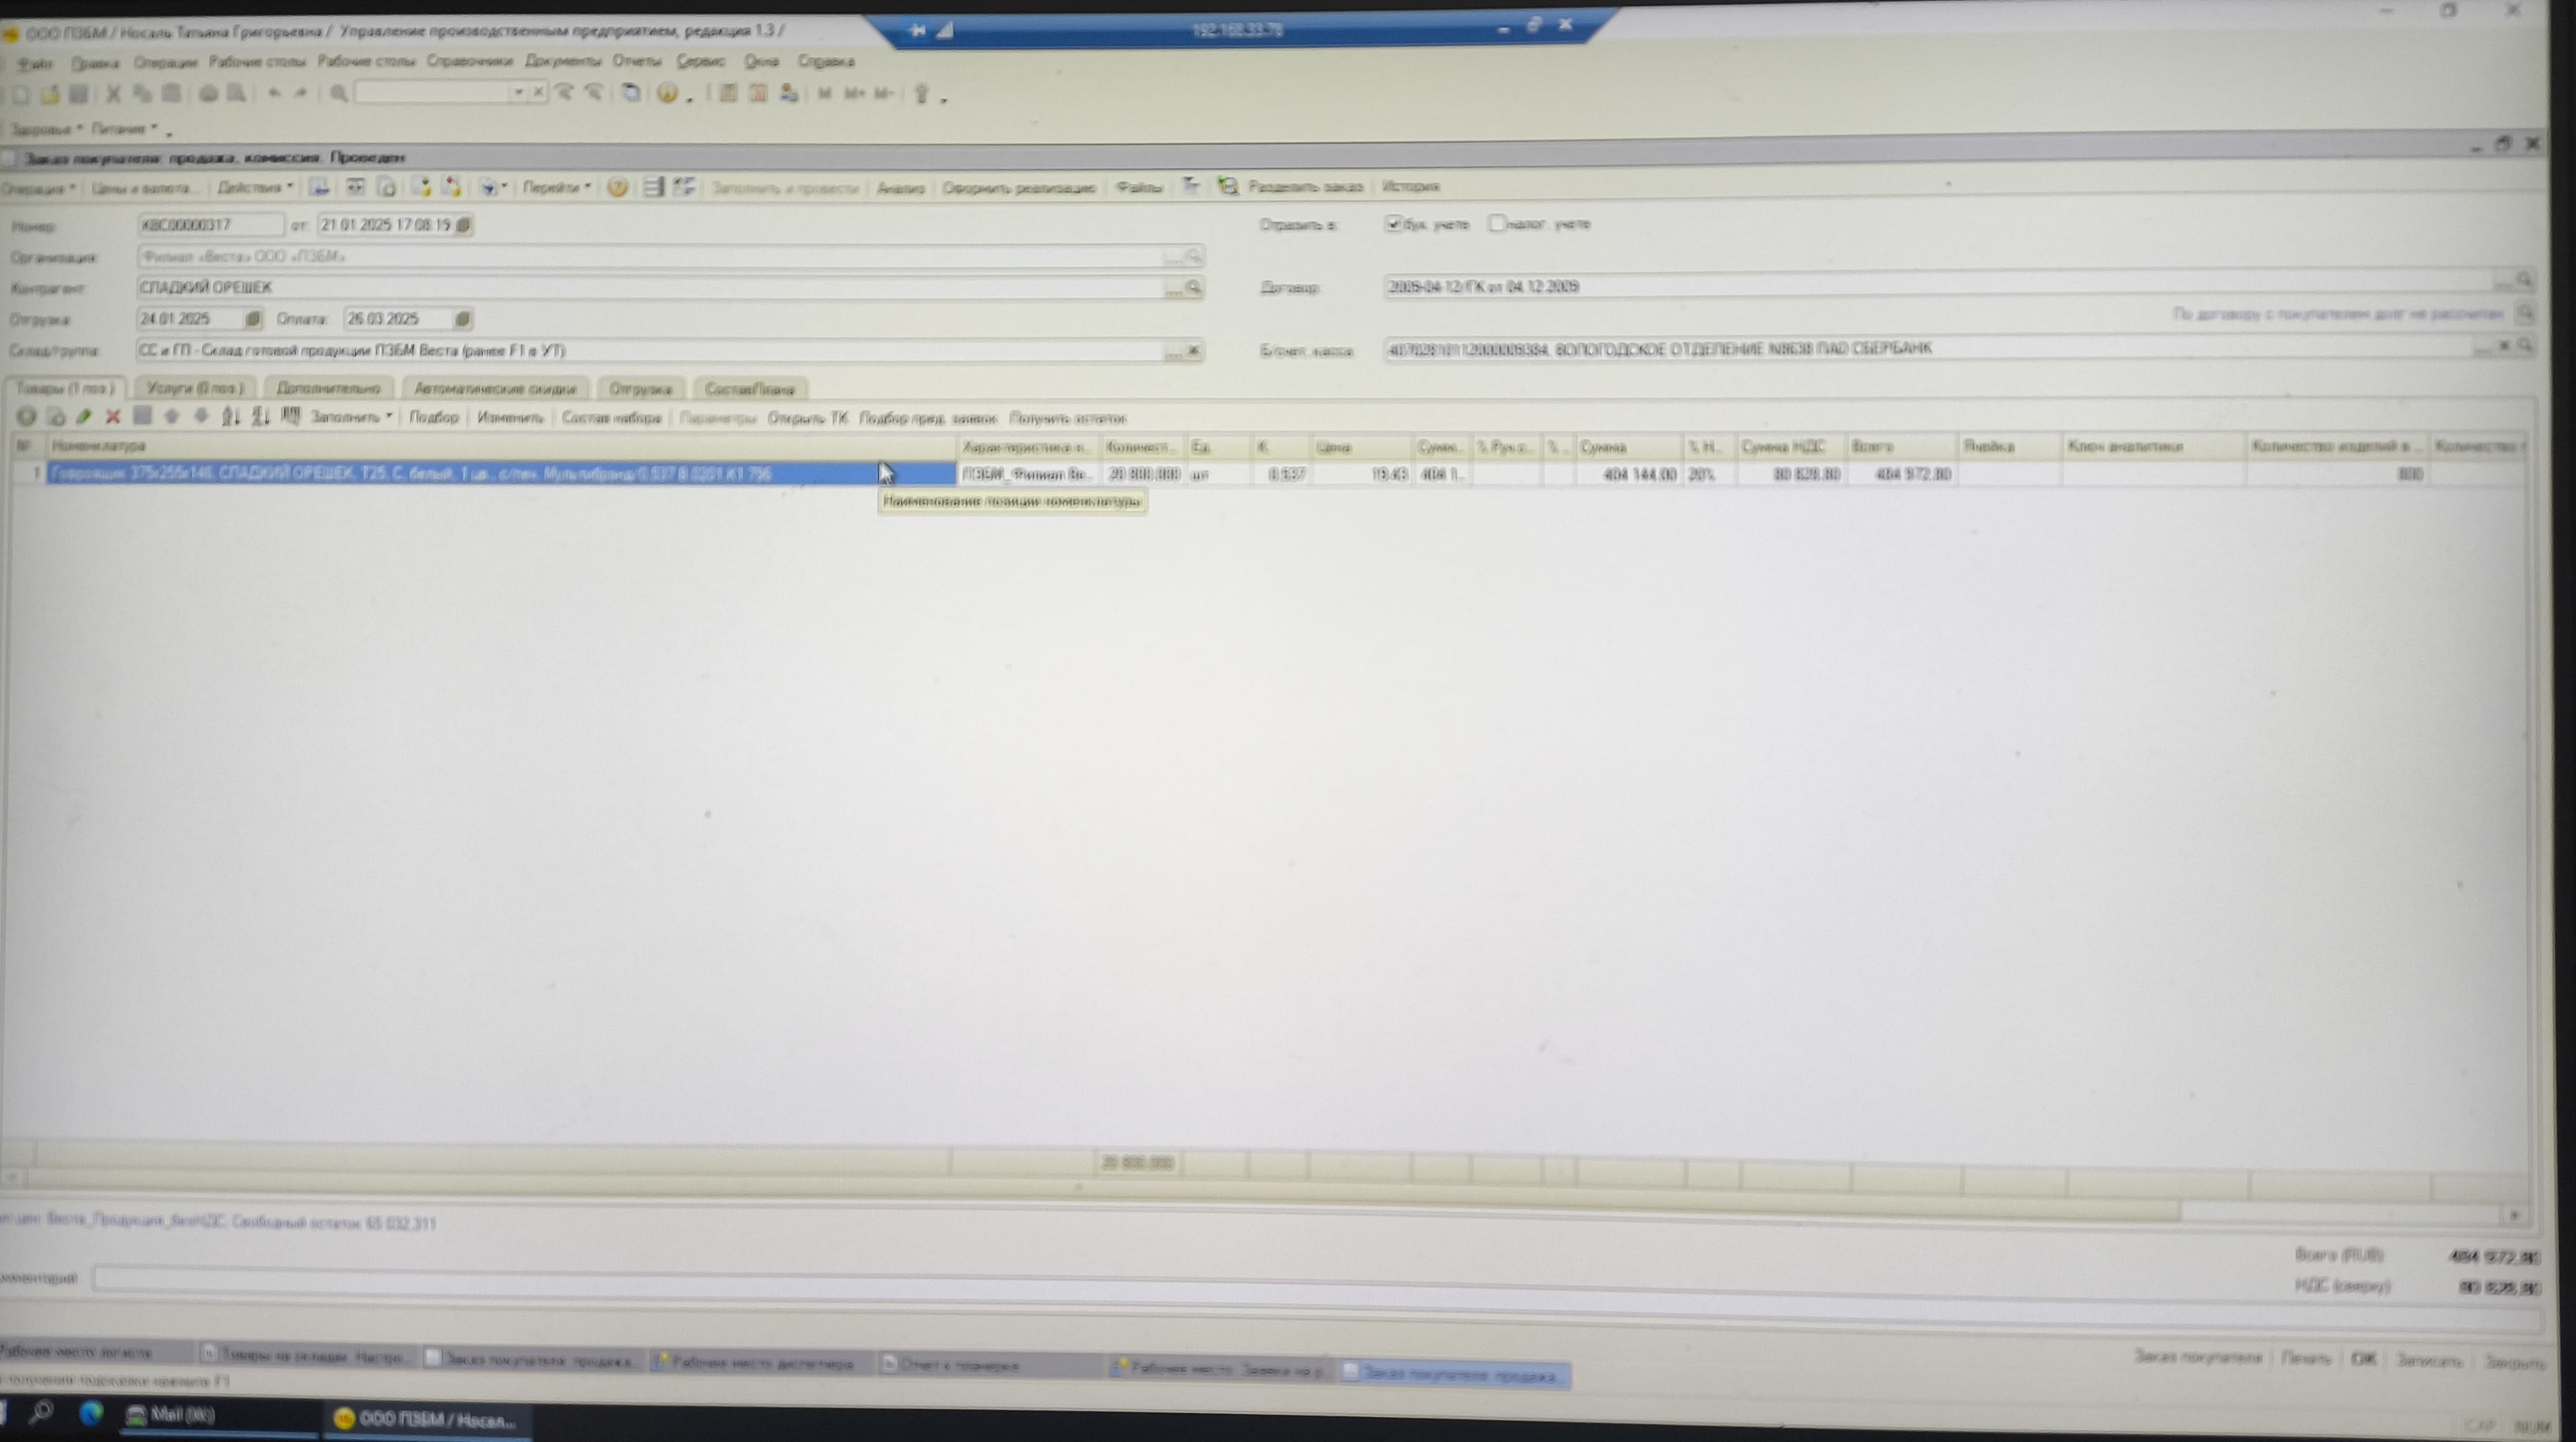
\includegraphics[height=0.35\textheight, keepaspectratio]{Pics/Х заказ покупателя.jpg}
\end{center}
 \caption{Заявка покупателя}
 \label{pic:Х заказ покупателя}
\end{figure}

\begin{figure}
\begin{center}
 \includegraphics[height=0.35\textheight, keepaspectratio]{Pics/Х вкладка отгрузка.jpg}
\end{center}
 \caption{Вкладка Отгрузка в заявке покупателя}
 \label{pic:Х вкладка отгрузка}
\end{figure}

\begin{figure}
\begin{center}
 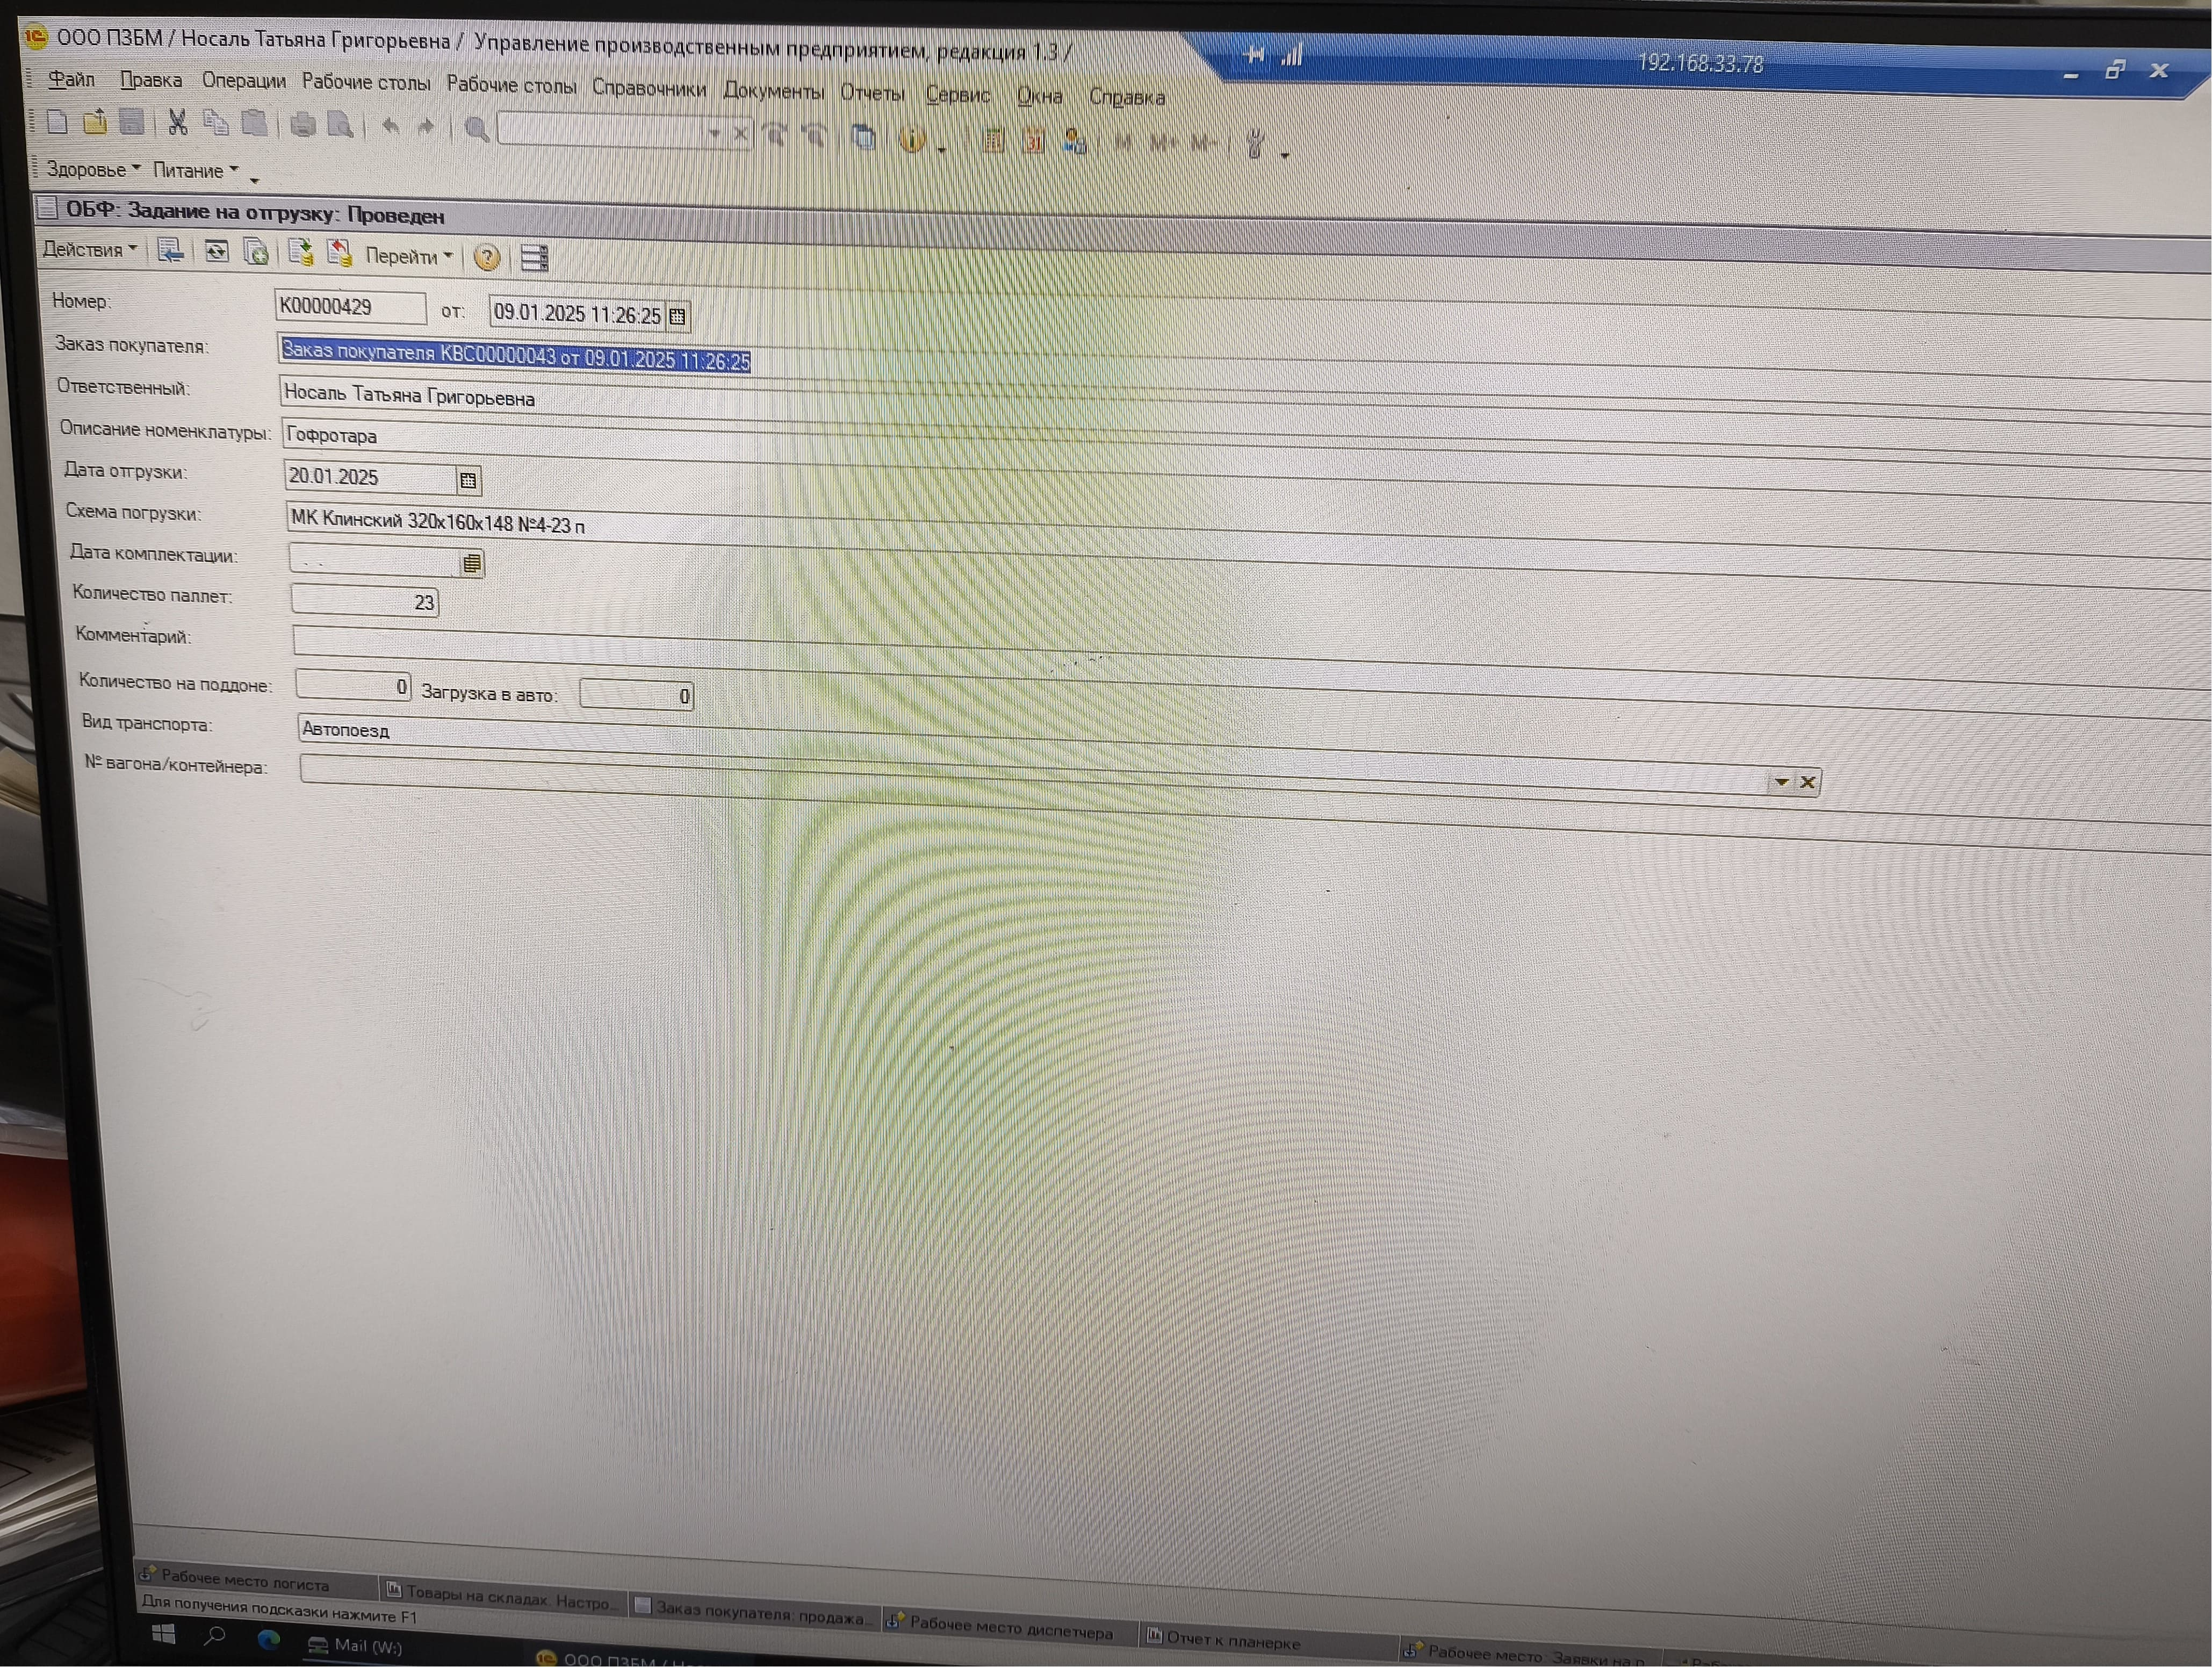
\includegraphics[height=0.45\textheight, keepaspectratio]{Pics/Х задание на отгрузку.jpg}
\end{center}
 \caption{Задание на отгрузку}
 \label{pic:Х задание на отгрузку}
\end{figure}


\begin{figure}
\begin{center}
 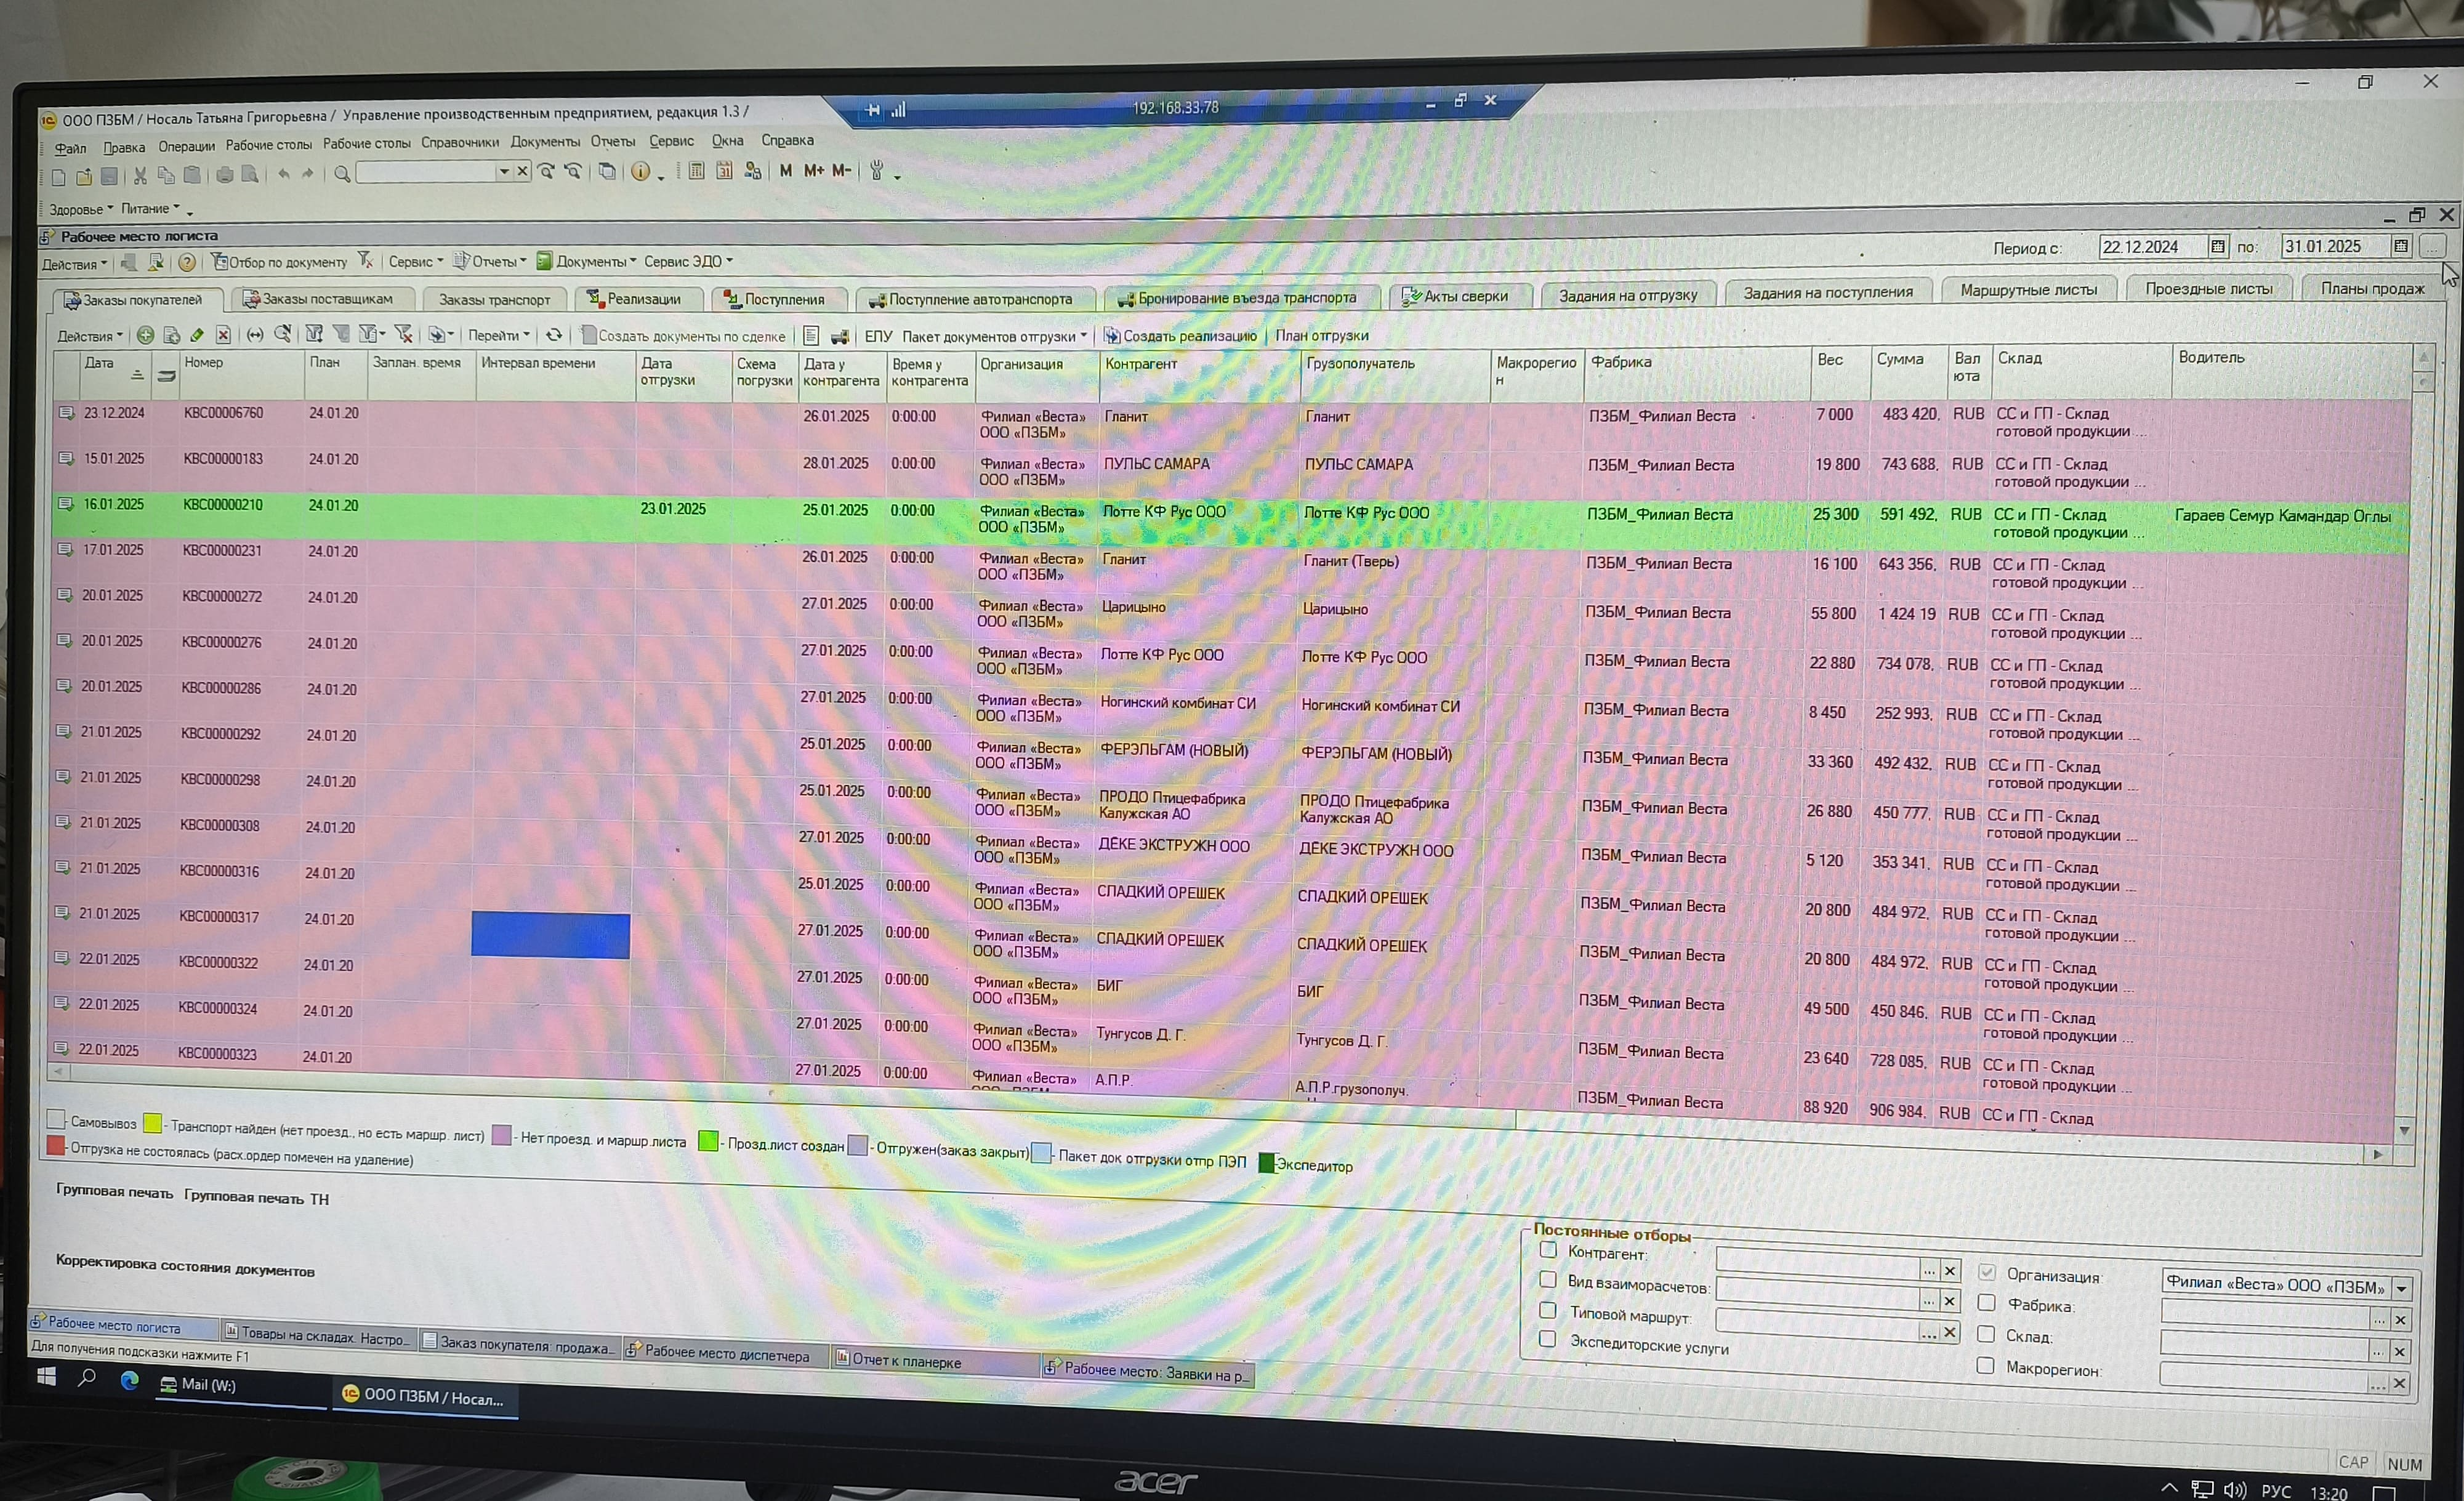
\includegraphics[height=0.4\textheight, keepaspectratio]{Pics/Х рабочее место логиста.jpg}
\end{center}
 \caption{Рабочий стол менеджера по логистике в 1С: УПП}
 \label{pic:Х рабочее место логиста}
\end{figure}

\begin{figure}
\begin{center}
 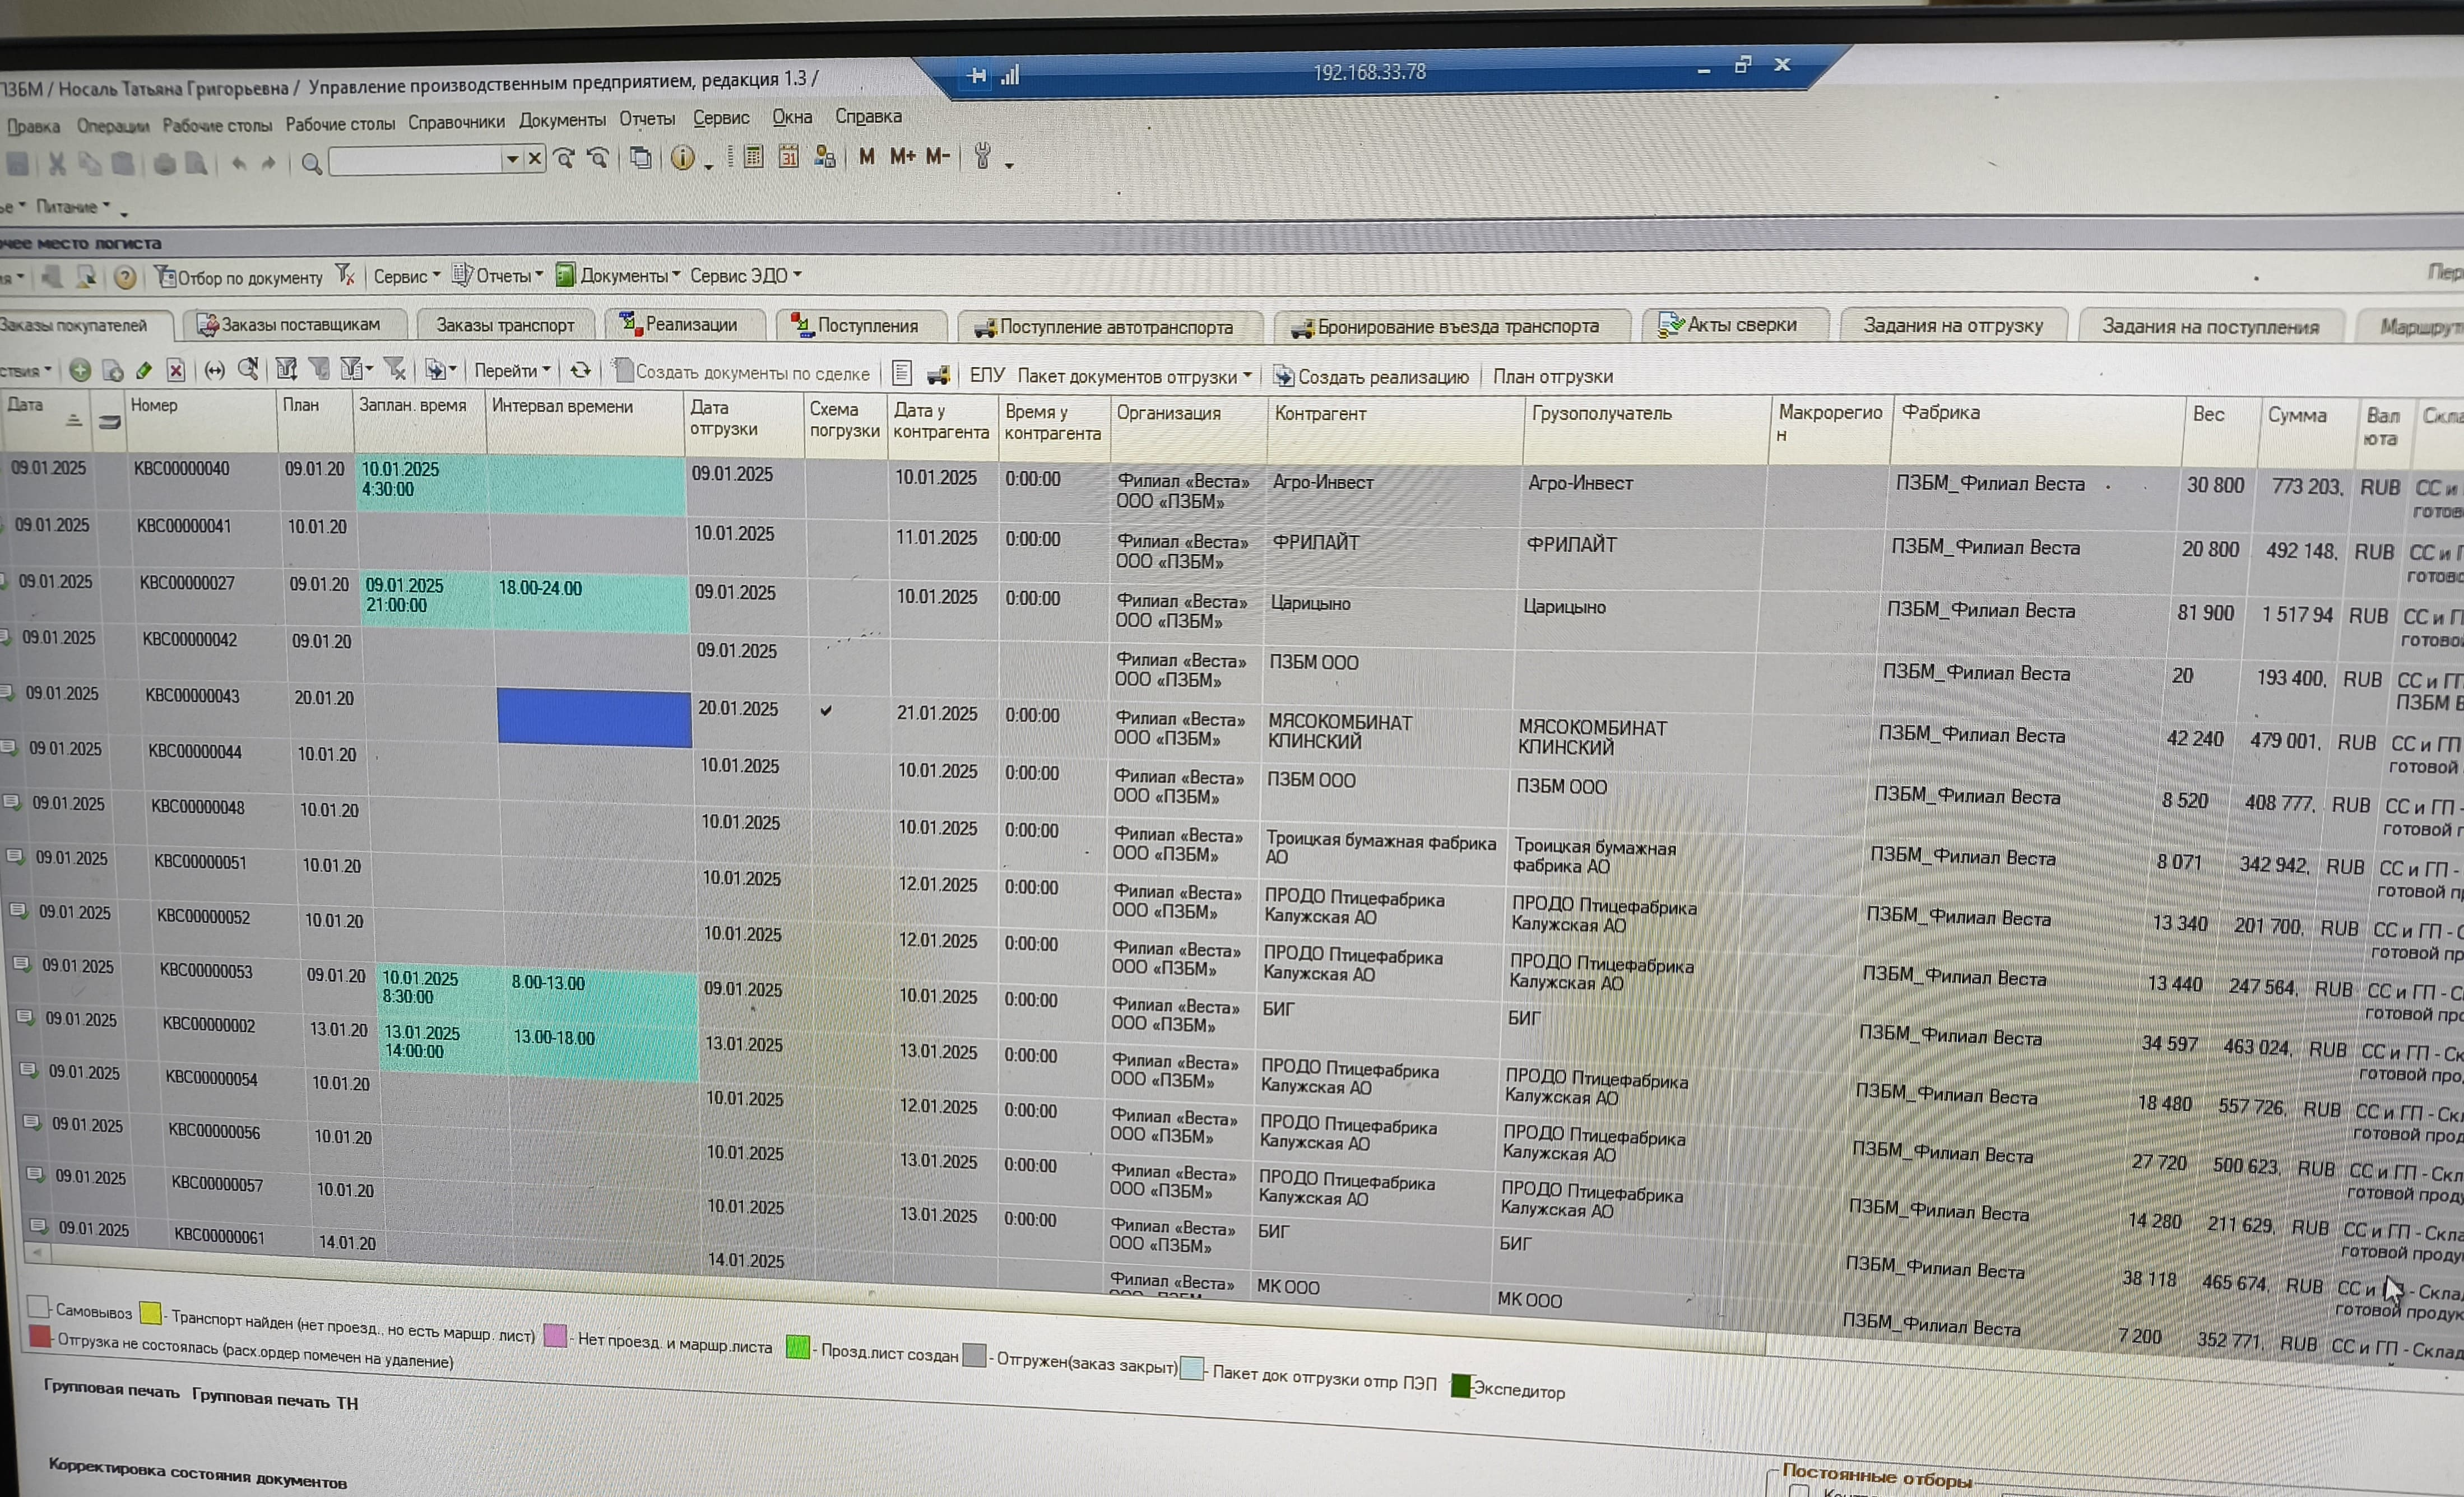
\includegraphics[height=0.4\textheight, keepaspectratio]{Pics/Х планирование отгрузок.jpg}
\end{center}
 \caption{Планирование отгрузки в 1С: УПП}
 \label{pic:Х планирование отгрузок}
\end{figure}

\begin{figure}
\begin{center}
 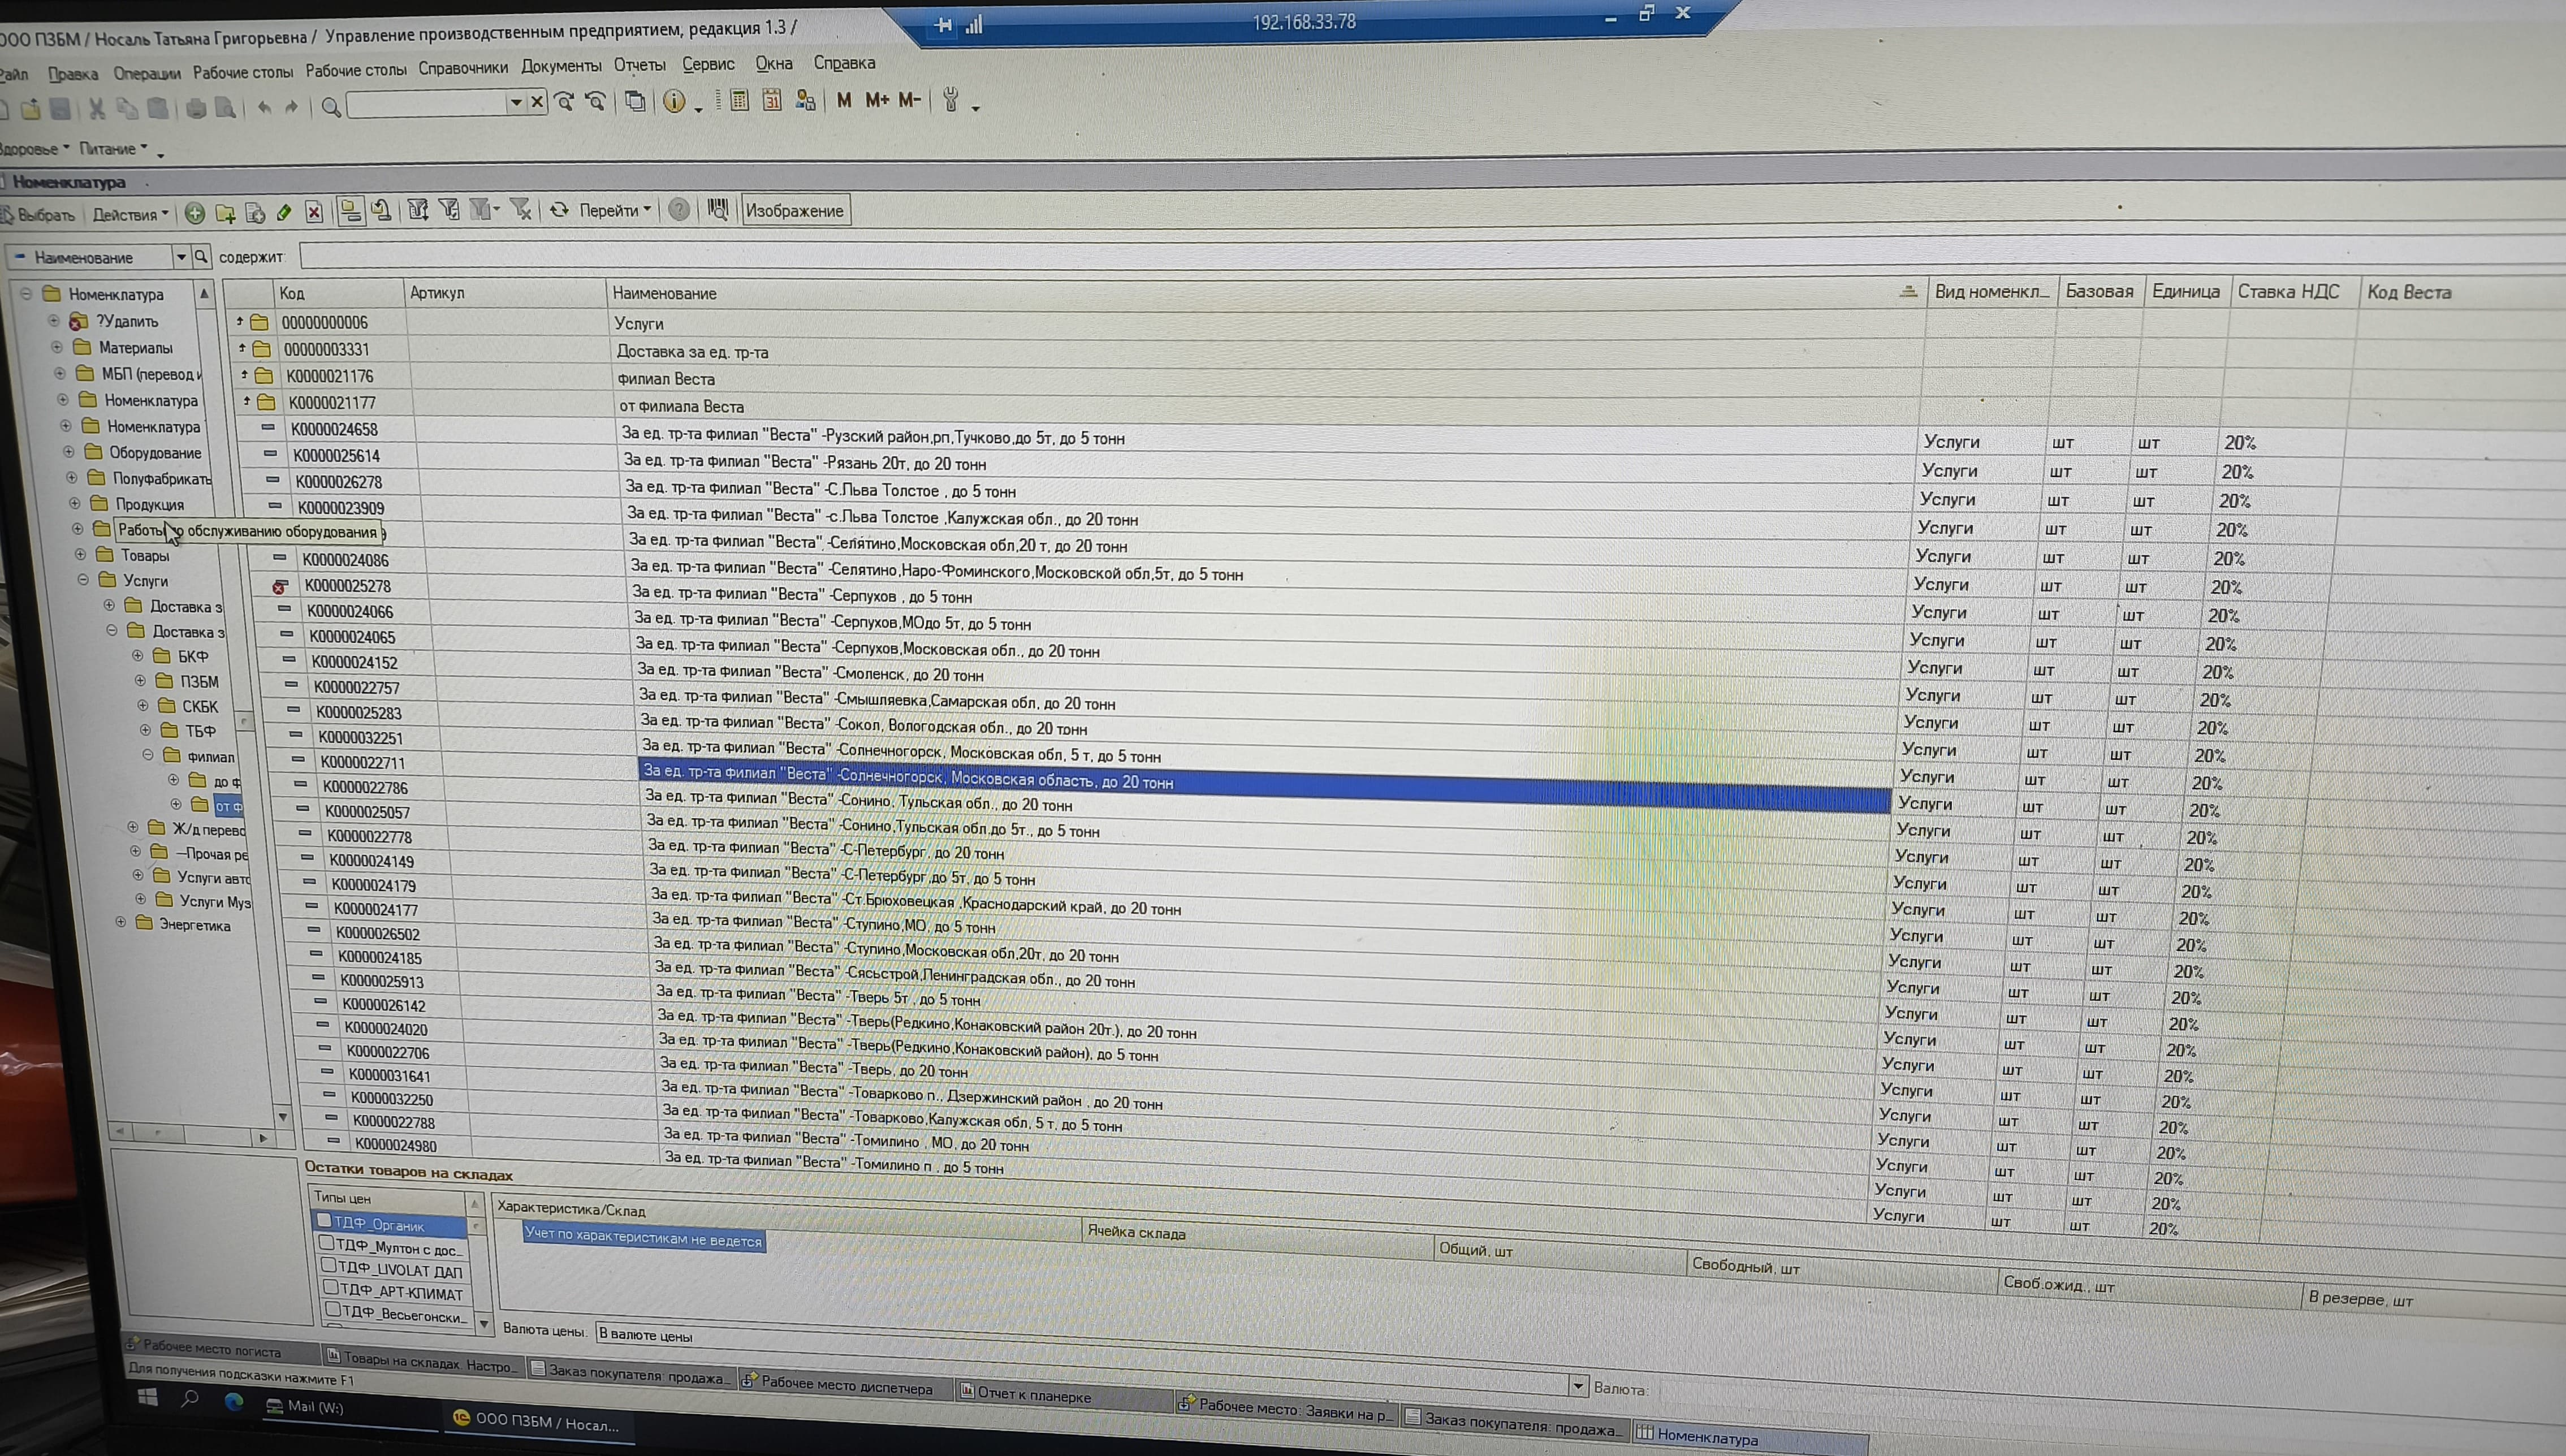
\includegraphics[height=0.3\textheight, keepaspectratio]{Pics/Х транспорт.jpg}
\end{center}
 \caption{Номенклатура доставки в 1С: УПП}
 \label{pic:Х транспорт}
\end{figure}


\begin{figure}
\begin{center}
 \includegraphics[height=0.35\textheight, keepaspectratio]{Pics/Х ЕЛУ.jpg}
\end{center}
 \caption{ЕЛУ (единый логистический узел) в 1С: УПП}
 \label{pic:Х ЕЛУ}
\end{figure}

\begin{figure}
\begin{center}
 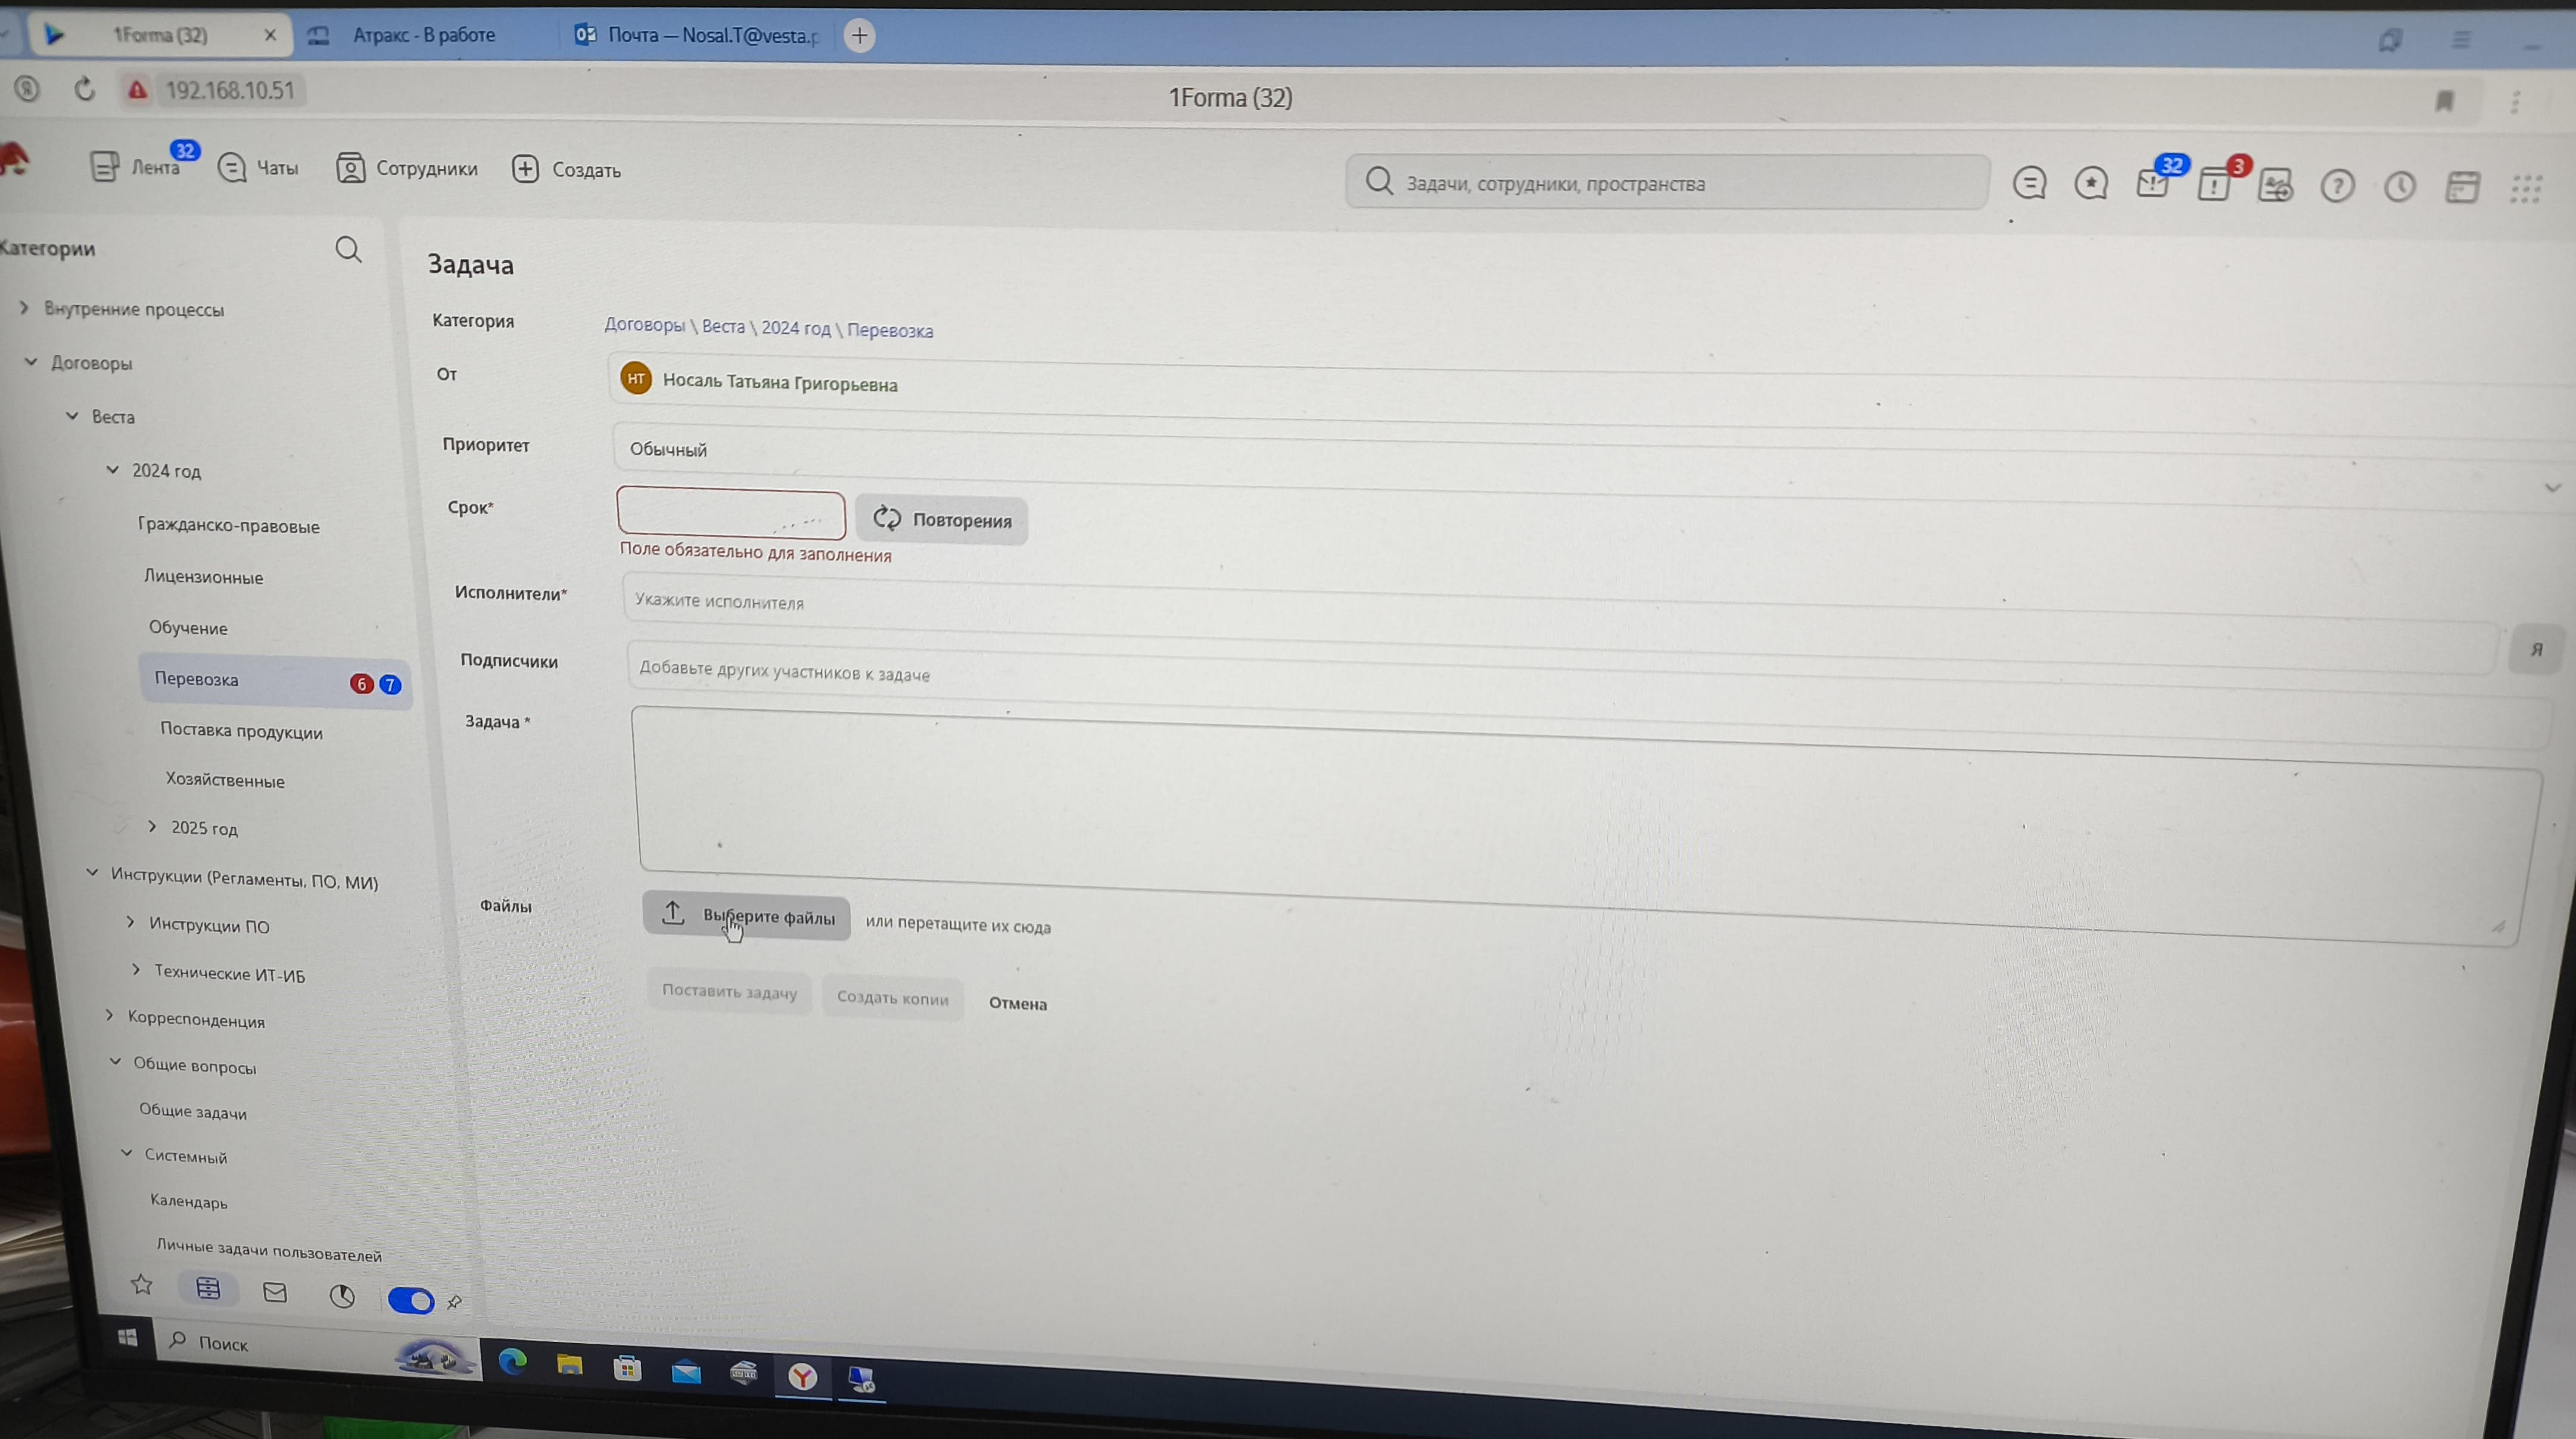
\includegraphics[height=0.35\textheight, keepaspectratio]{Pics/Х первая форма.jpg}
\end{center}
 \caption{Первая форма у логиста}
 \label{pic:Х первая форма}
\end{figure}

\begin{figure}
\begin{center}
 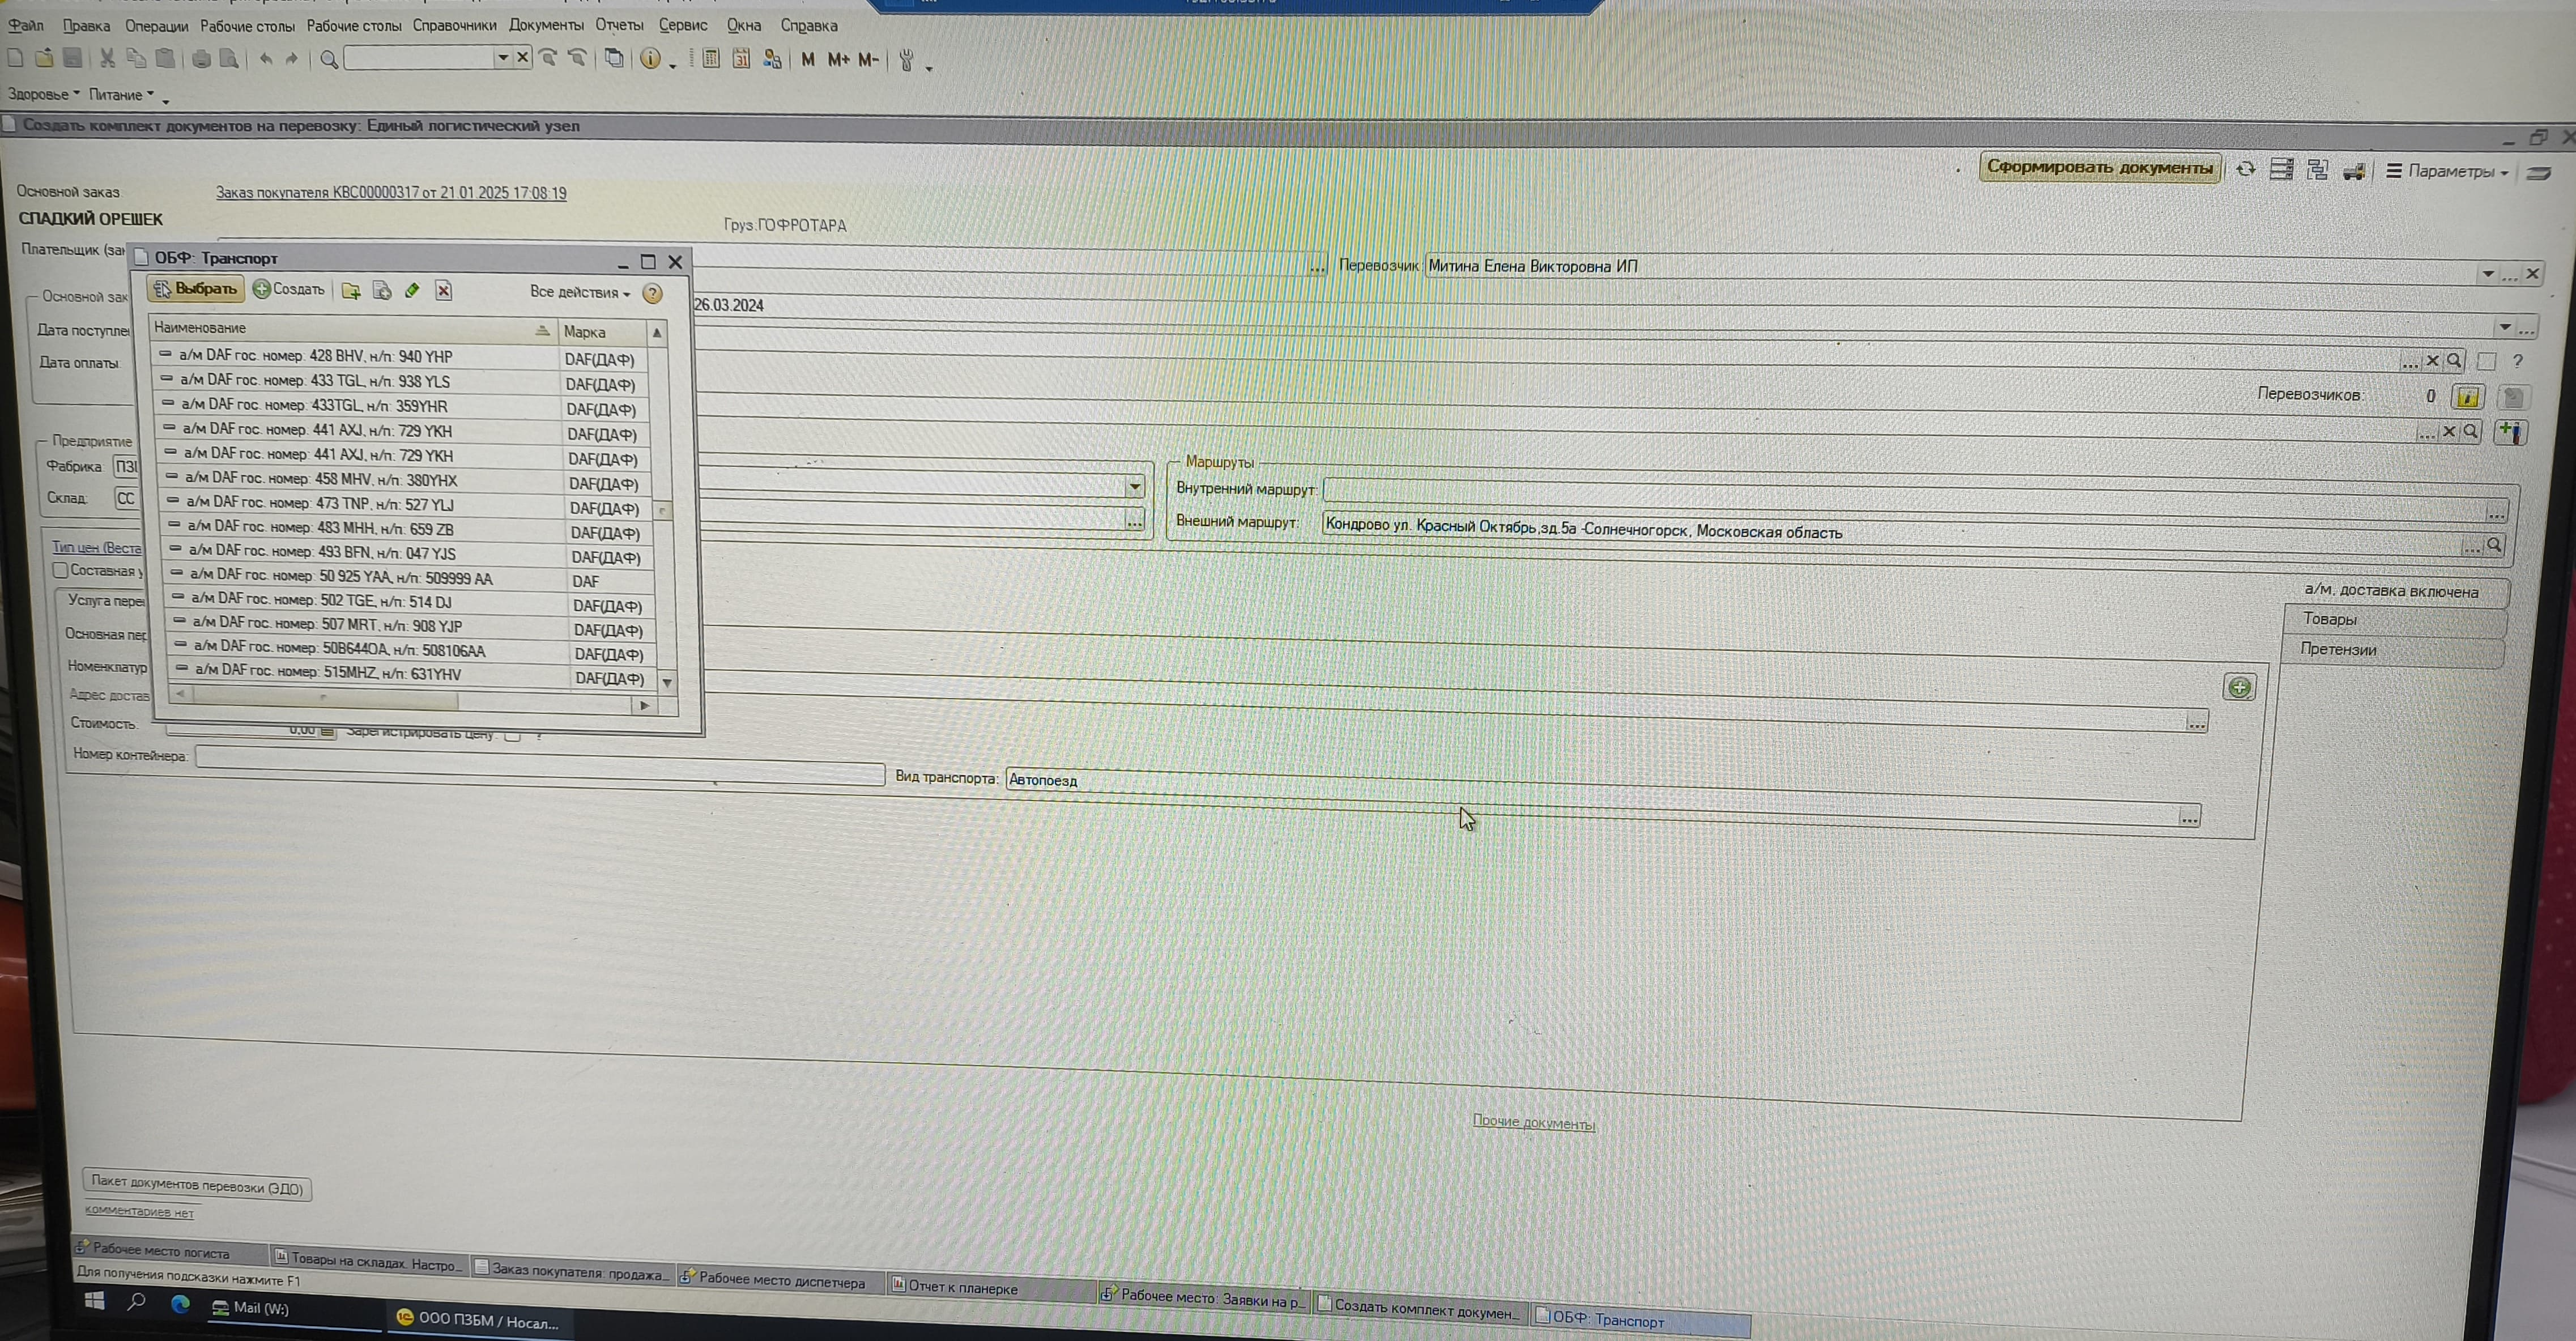
\includegraphics[height=0.3\textheight, keepaspectratio]{Pics/Х справочник транспорта.jpg}
\end{center}
 \caption{Справочник транспорта в 1С: УПП}
 \label{pic:Х справочник транспорта}
\end{figure}

\begin{figure}
\begin{center}
 \includegraphics[height=0.4\textheight, keepaspectratio]{Pics/Х схемы погрузки.jpg}
\end{center}
 \caption{Вид формы создания схемы погрузки в автотранспорт}
 \label{pic:Х схемы погрузки}
\end{figure}

\begin{figure}
\begin{center}
 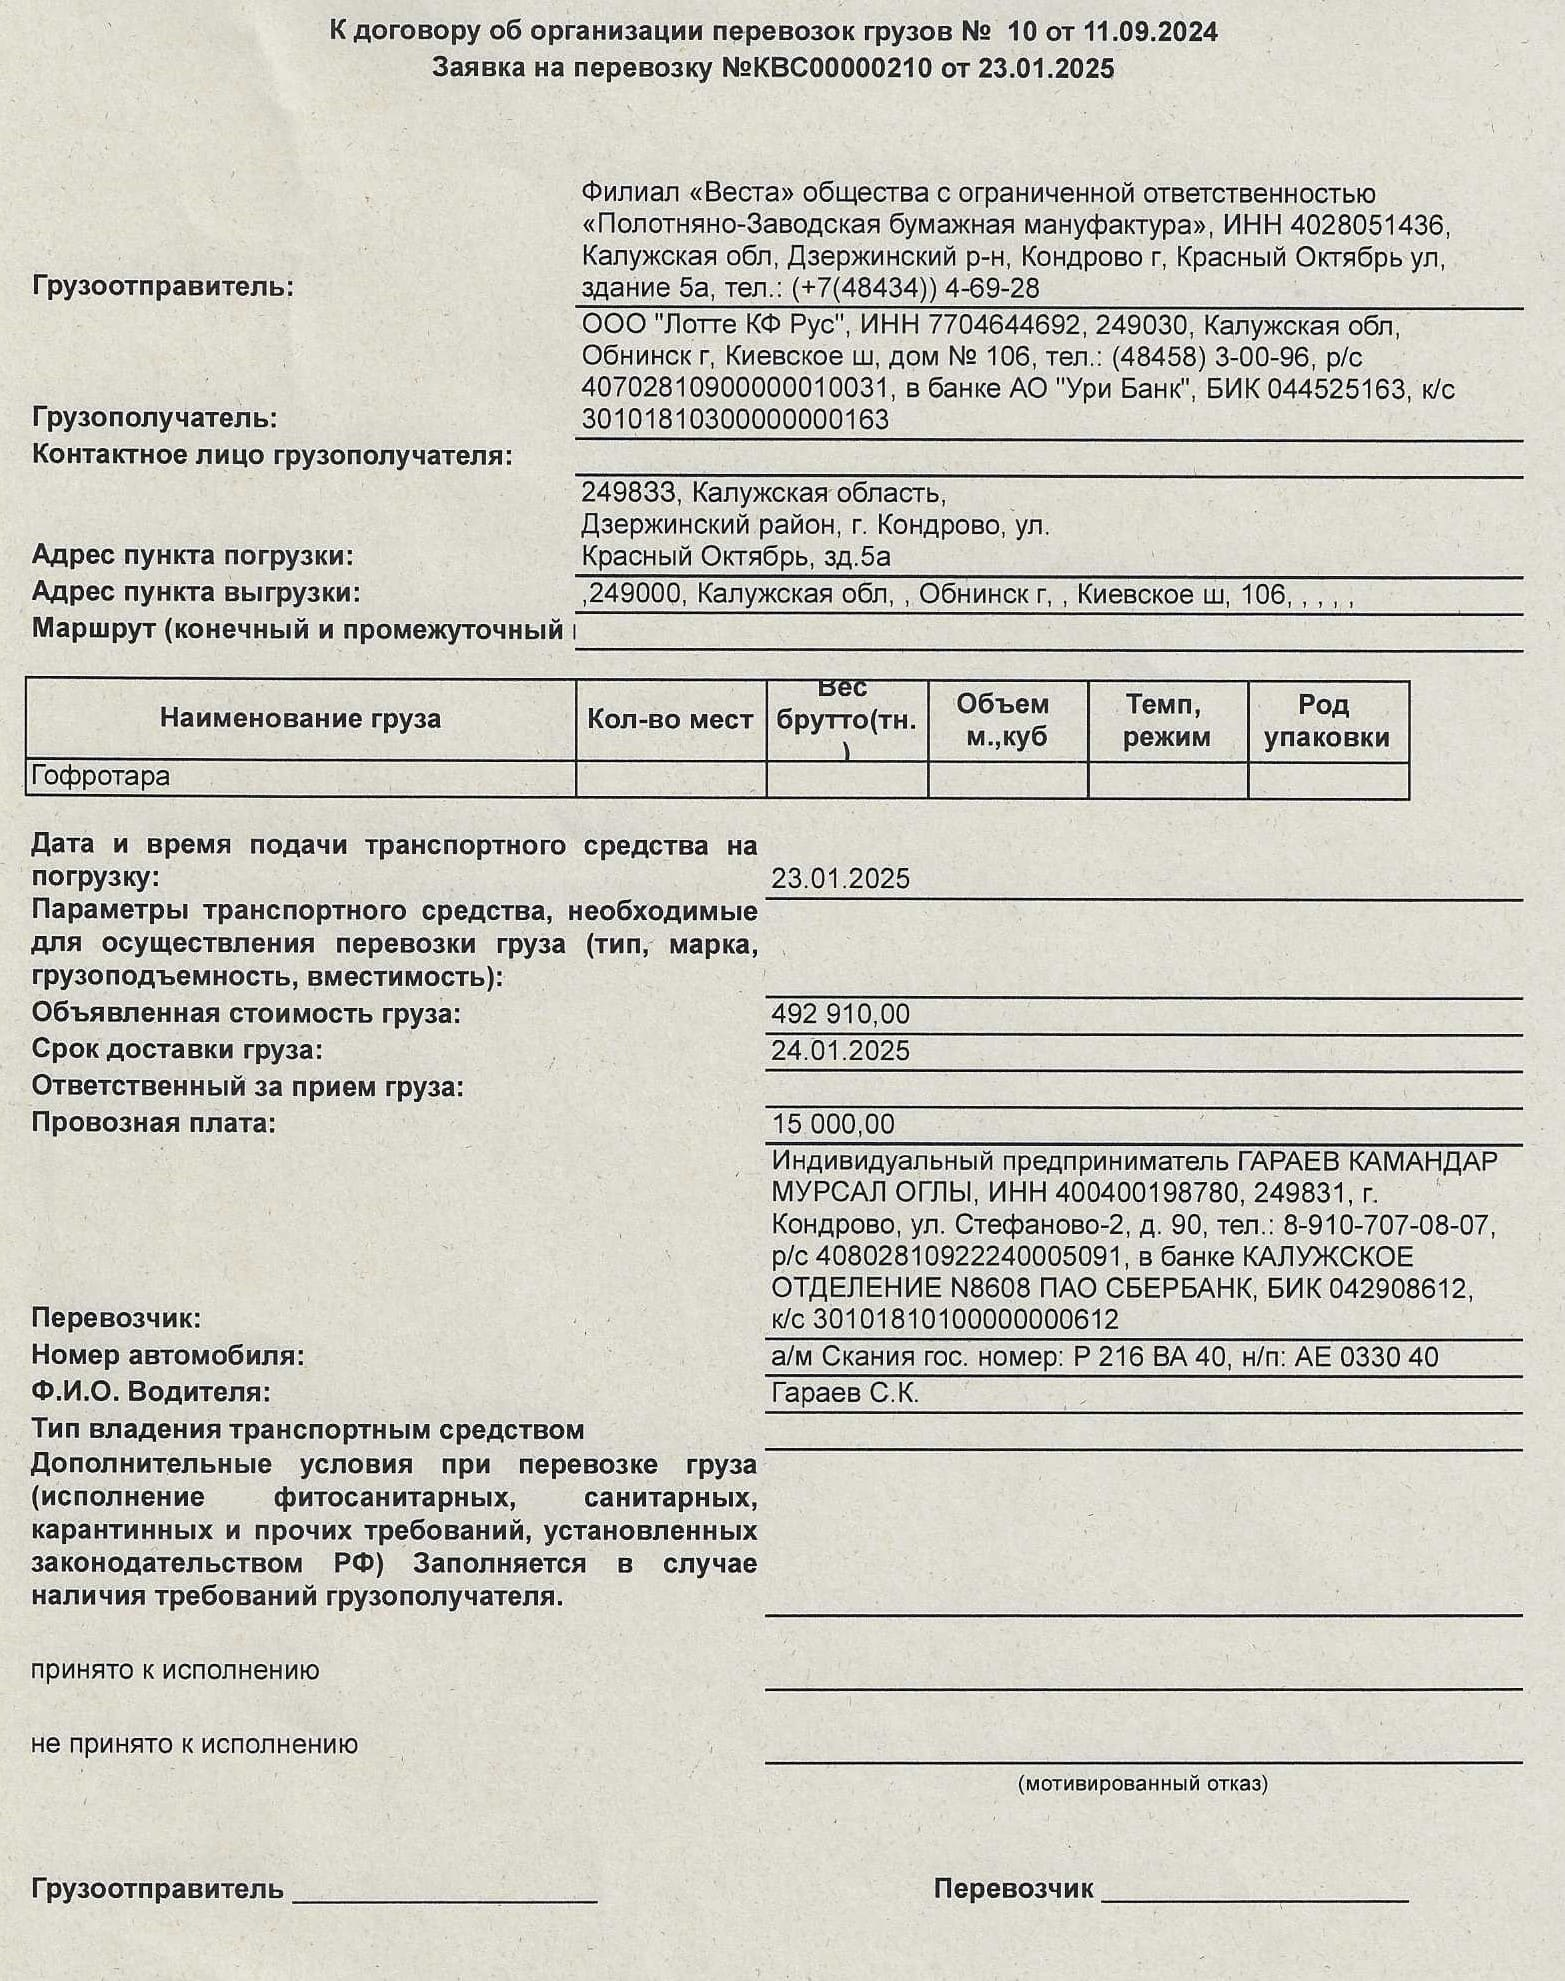
\includegraphics[height=0.8\textheight, keepaspectratio]{Pics/X.1.jpg}
\end{center}
 \caption{Форма заявки на перевозку}
 \label{pic:X.1}
\end{figure}

\begin{figure}
\begin{center}
 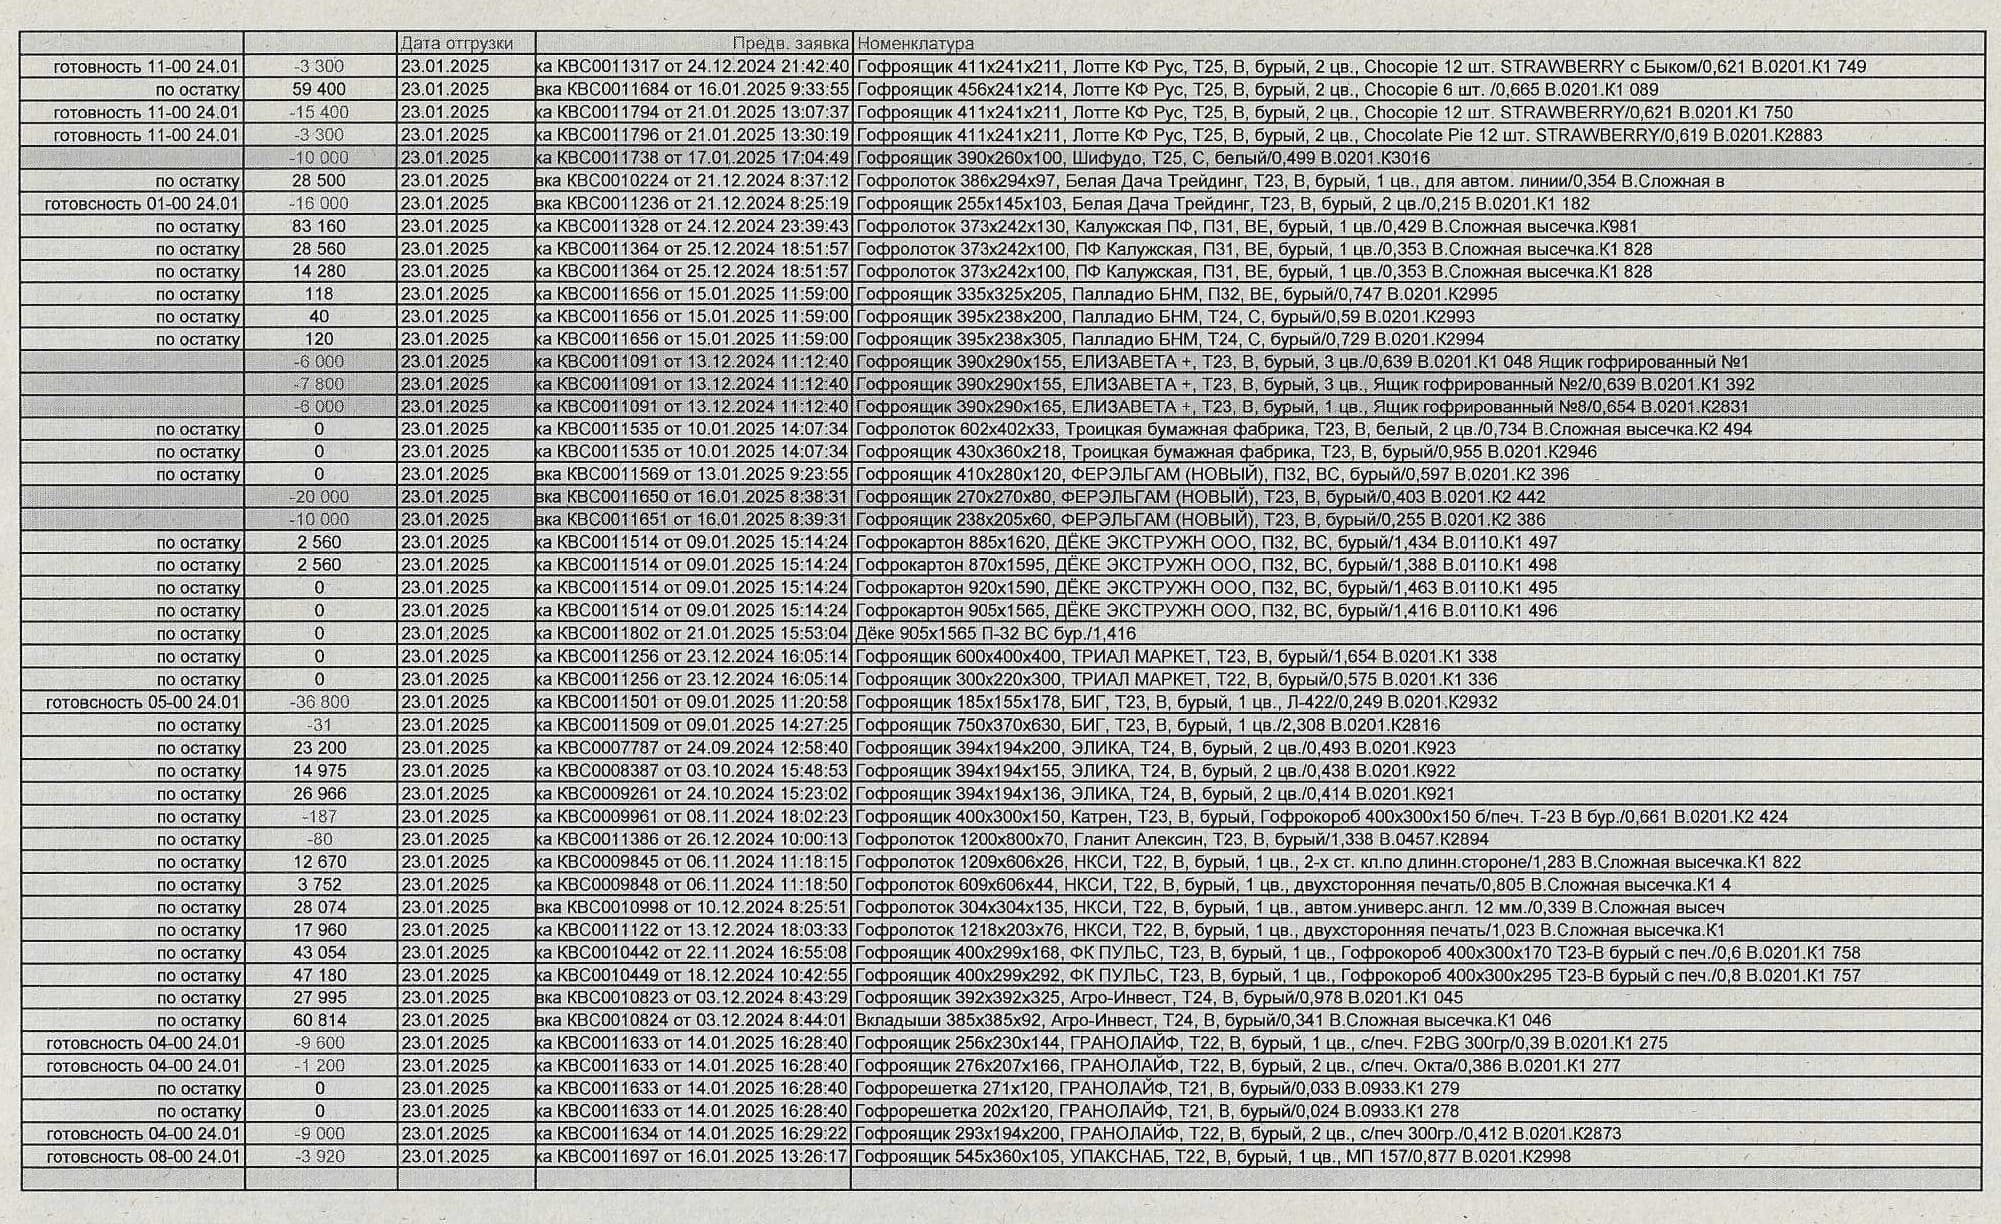
\includegraphics[height=0.5\textheight, angle=90, keepaspectratio]{Pics/X.8.jpg}
\end{center}
 \caption{Подтвержденный план отгрузки от отдела планирования}
 \label{pic:X.8}
\end{figure}

\begin{figure}
\begin{center}
 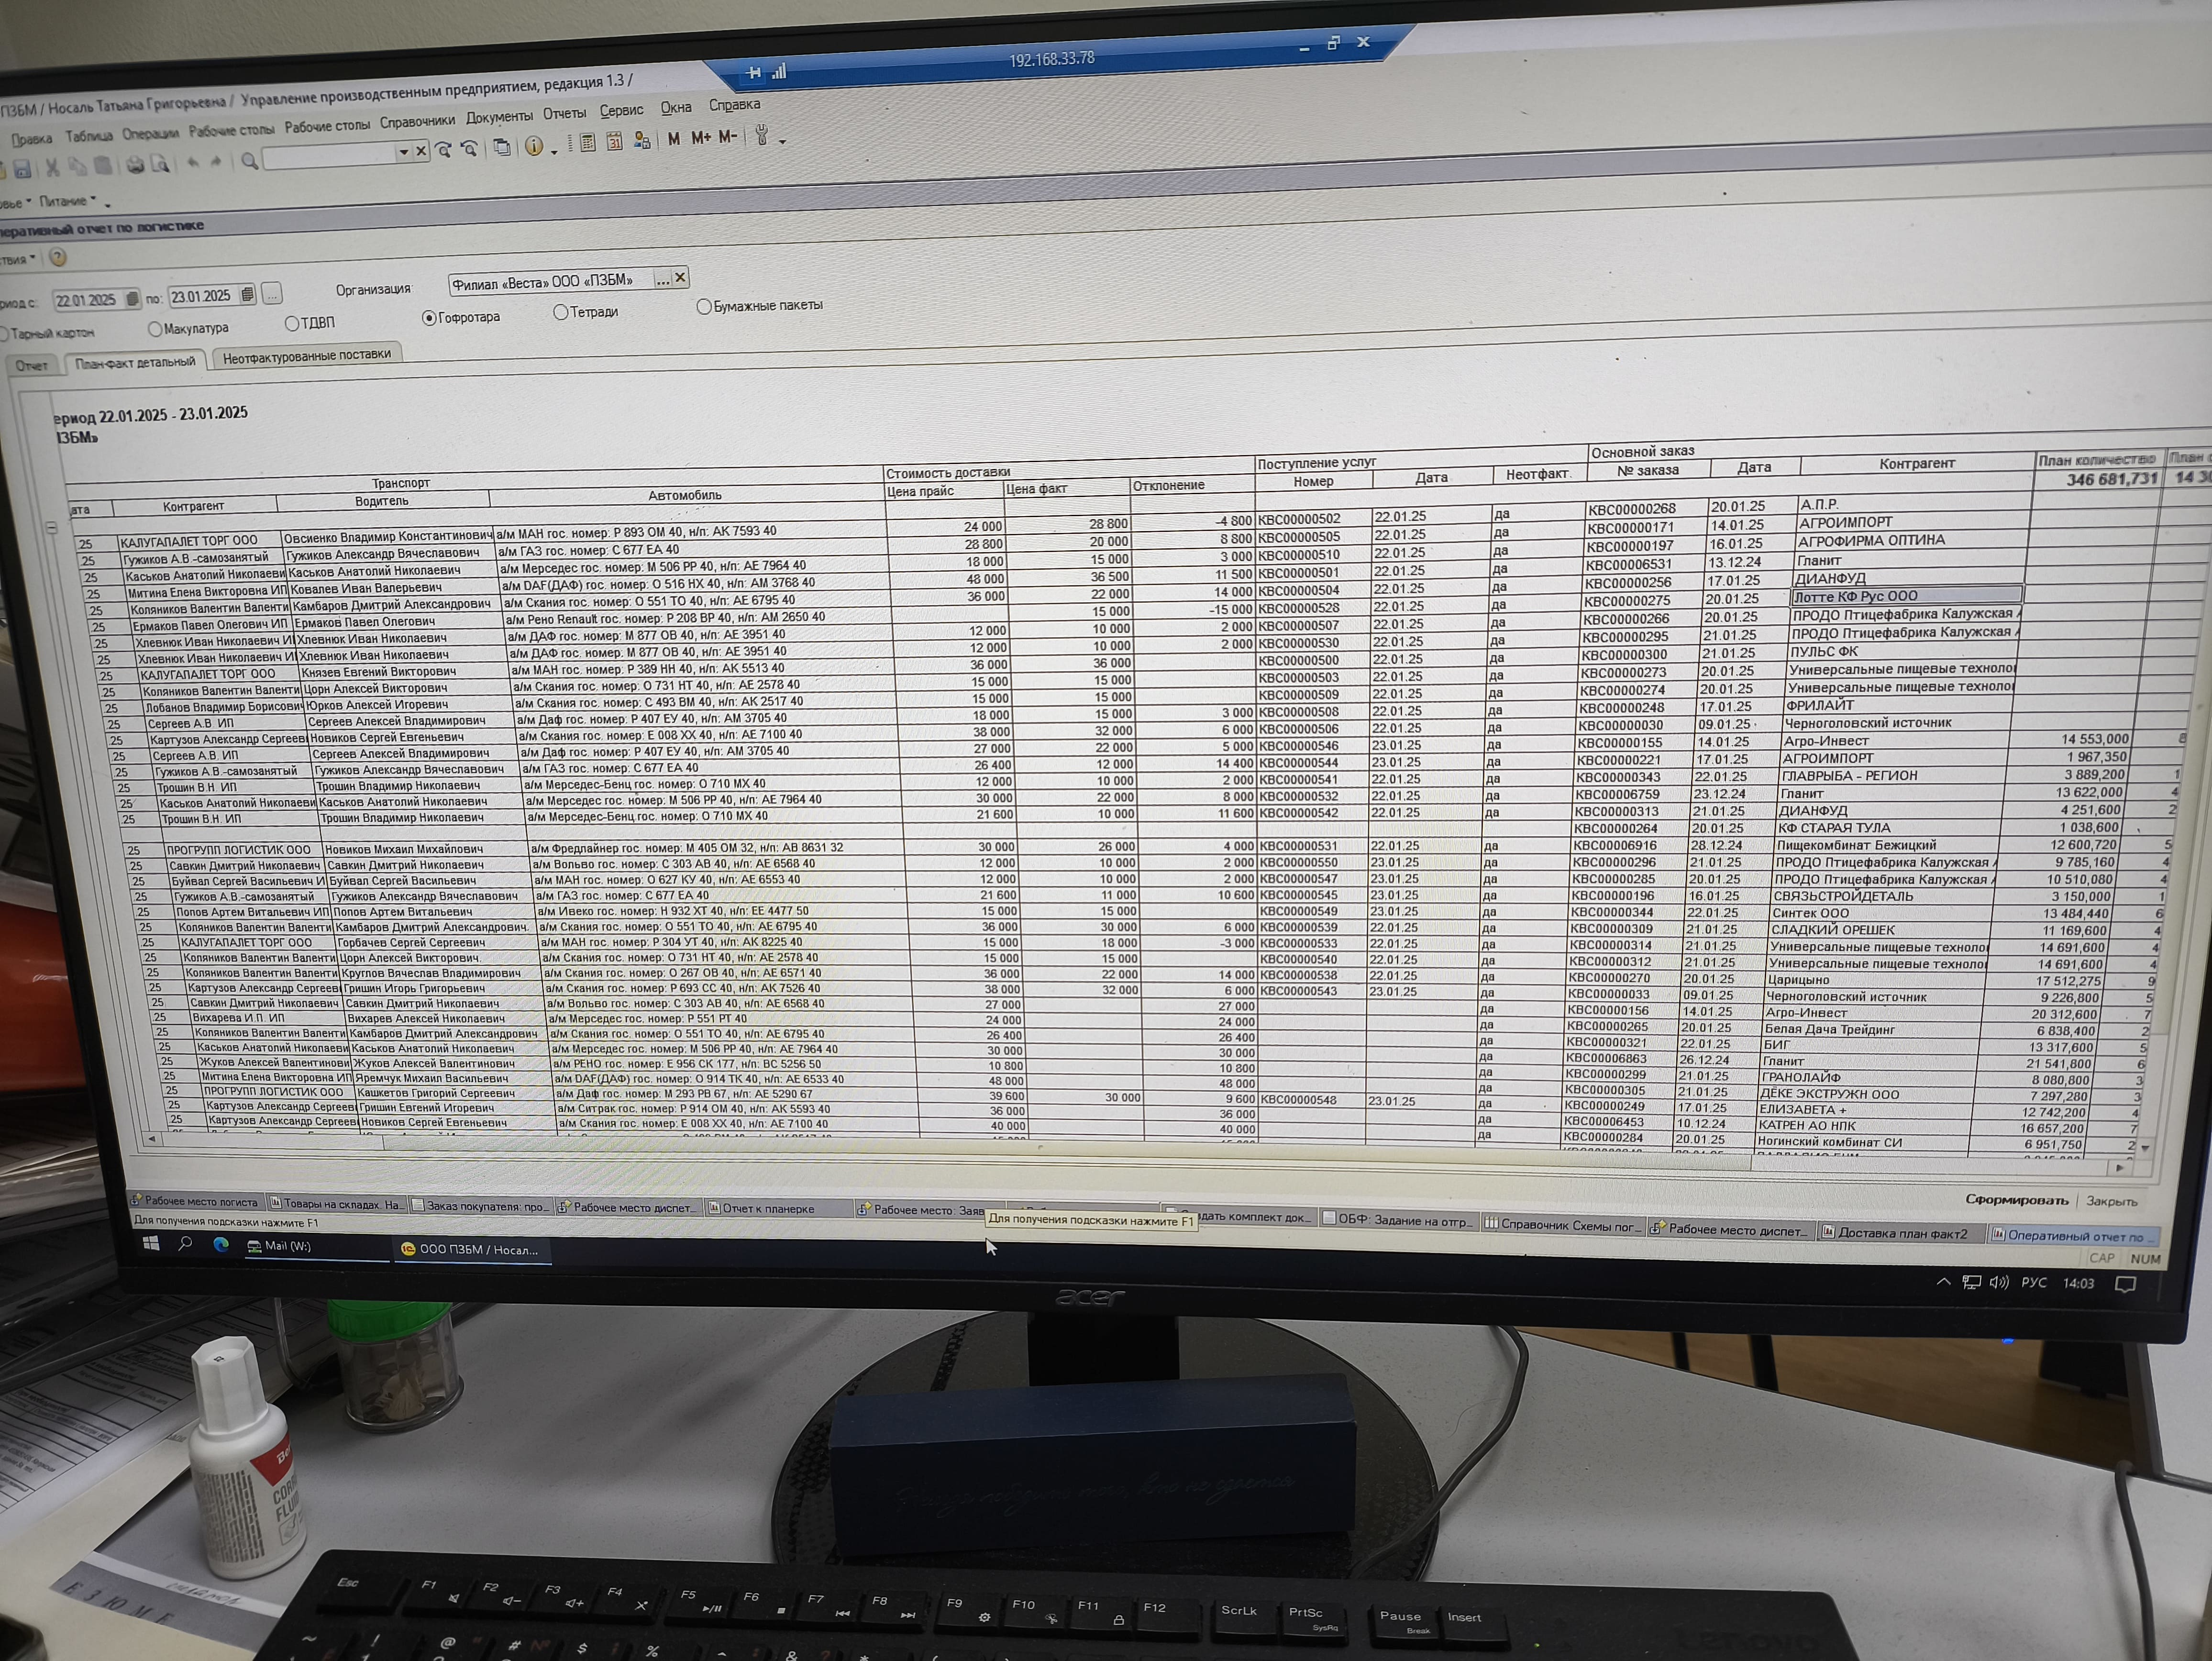
\includegraphics[height=0.4\textheight, keepaspectratio]{Pics/Х отчет по логистике.jpg}
\end{center}
 \caption{Оперативный отчет по логистике в 1С: УПП}
 \label{pic:Х отчет по логистике}
\end{figure}

\clearpage
%Каждое утро менеджер видит остатки по готовой продукции на складах в системе СБИС (отчет по остаткам). Менеджер пишет задание на отгрузку в чат mail.ru инженерам по отгрузке и формирует заявку (рис. \ref{pic:d22}).

%В СБИС инженер по отгрузке создает план отгрузки (рис. \ref{pic:d22}). 
%Предприятие использует только наемный транспорт или самовывоз транспортом заказчика.
%Менеджер создает план отгрузки  (рис. \ref{pic:d23}) в конце рабочего дня с опозданием на 6 часов и передает в производство мастеру и на склад.
%План отгрузки передается мастеру производства.

%На основании плана отгрузки (рис. \ref{pic:d23}) инженер по отгрузке создает распоряжение на отгрузку в СБИС (рис. \ref{pic:d24}).


% Каждый день до 16:00 (?) МСЗ по плану производства из таблицы MS Excel планирует отгрузку в соответствии с планом производства на основании списка заказов покупателей и остатков ГП (рис. \ref{pic:d17}).
% , \ref{pic:d8}) 
%Отгрузки согласовываются с клиентом. %Менеджер планирует отгрузку (рис. \ref{pic:d17}). 


% Каждый менеджер на основании плана отгрузки (рис. \ref{pic:d17}) пишет заявку на отгрузку (рис. \ref{pic:d10}). 
%Менеджер пишет в чате или сообщает устно логисту о созданном распоряжении.
%Начальник отдела логистики в чате получает пожелания от менеджеров по отгрузке. Почти вся продукция отгружается  на поддонах.
%Начальник отдела логистики получает заявку (рис. \ref{pic:d24}) в системе СБИС.
%На предприятии выделен 1 логист (Начальник отдела логистики). Начальник отдела логистики ищет машины, создает подачи график машин.

%Начальник отдела логистики по заявке на продажу подбирает транспорт.
% и планирует подачу транспорта на предприятие, разрабатывает график отгрузки. Заявка на отгрузку создается за два дня до отгрузки.
%Начальник отдела логистики составляет план суточный по отгрузке. Время подачи машины не указывается.
% Для поиска машин для межгорода логисты используют сервис Ati.ru.

%Начальник отдела логистики считает загрузку на фуру по техкарте упаковки (рис. \ref{pic:d26_1}). Начальник отдела логистики создает заявку на транспорт в СБИС (рис. \ref{pic:d27}), вручную заносит в форму плана отгрузки MS Excel (рис. \ref{pic:d25}), передает менеджеру и на склад кладовщикам
%в системе СБИС на основе заявки на транспорт. Начальник отдела логистики указывает водителя и машину в форме \ref{pic:d24}).

%Начальник отдела логистики пишет заявку перевозчику по емайл или по телефону. 
%Факт отгрузки Начальник отдела логистики смотрит по данным системы СБИС, проверяет факт отгрузки готовой продукции.
 

%Инженер по отгрузке в системе СБИС формирует пропуск (распоряжение на отгрузку), указывает машину из формы \ref{pic:d25} в СБИС.

% %\begin{figure}
% \begin{center}
%   \includegraphics[height=0.94\textheight, width=\textwidth, keepaspectratio]{Pics/d24.jpg}
% \end{center}
%   \caption{Распоряжение на отгрузку в СБИС}
%   \label{pic:d24}
% \end{figure}



% \begin{figure}
% \begin{center}
%   \includegraphics[height=0.8\textheight, width=\textwidth, keepaspectratio]{Pics/d25.jpg}
% \end{center}
%   \caption{План отгрузки готовой продукции}
%   \label{pic:d25}
% \end{figure}

% \begin{figure}
% \begin{center}
%   \includegraphics[height=0.94\textheight, width=\textwidth, keepaspectratio]{Pics/d26_1.jpg}
% \end{center}
%   \caption{Технологическая карта на отгрузку}
%   \label{pic:d26_1}
% \end{figure}

% \begin{figure}
% \begin{center}
%   \includegraphics[height=0.94\textheight, width=\textwidth, keepaspectratio]{Pics/d27.jpg}
% \end{center}
%   \caption{Форма заявки на транспорт в СБИС}
%   \label{pic:d27}
% \end{figure}


%Менеджеры отдела продаж контролируют выпуск готовой продукции по появлению остатков ГП. Контроль остатков ведется в файле MS Excel \ref{pic:11_stockGPexcel}. 
%Остатки по ГП актуальны на следующий день после производства к 10:00. 
%Поскольку на предприятии выделены два юридических лица, то менеджеры контролируют остатки по ГП по обеим юридическим лицам. 
%
%Менеджеры отдела продаж ведут файл плана отгрузки \ref{pic:10_shipping_plan1} в электронном виде в формате Excel.
%План отгрузки менеджер формирует на основании заявок на производство \ref{pic:09_OrederToProduction}, где указана желаемая и согласованная дата отгрузки.
%
%План отгрузки в электронном виде находится в сетевом доступе.
%Согласованный план отгрузки менеджер передает логисту для планирования транспорта.
%
%Логист постоянно контролирует файл плана отгрузки \ref{pic:10_shipping_plan1}, определяет на основании плана отгрузки транспорт и формирует план отгрузки с учетом поставки транспорта \ref{pic:10_shipping_plan2}. 
%Логист корректирует планы отгрузки \ref{pic:10_shipping_plan2}, указывает транспортное средство и время прибытия, адреса доставки.
%На предприятии существует собственный транспорт. В сутки собственный транспорт делает от 4 до 10 поездок.
%Согласованный логистом план отгрузки передается на склад в электронном виде через сетевой каталог.
%
%На основании плана отгрузки \ref{pic:10_shipping_plan2} логист формирует заявки сторонним экспедиторам на поставку транспорта \ref{pic:12_application_for_forwarder}, которые отправляются по электронной почте. Логист должен заказать автотранспорт за один-два дня до отгрузки.
%
%Выделены отгрузка авто и жд транспортом (контейнеры). В месяц формируется до 8 контейнеров с ГП. При контейнерной отгрузке  логист должен заказывать у логистической компании контейнер за 10 дней до отгрузки. 
%
%
%
%Менеджер контролирует отгрузку в программе 1С по отчету по продажам либо по журналу реализации. Менеджер корректирует планы отгрузки по факту отгрузки.
%
%
% \begin{figure}
% \begin{center}
%  \includegraphics[width=\linewidth, height=0.94\textheight, keepaspectratio]{Pics/d22.jpg}
% \end{center}
%  \caption{Список заказов  для отгрузки}
%  \label{pic:d22}
% \end{figure}

% % \begin{figure}
% % \begin{center}
% %  \includegraphics[width=\linewidth, height=0.94\textheight, keepaspectratio]{Pics/d22.jpg}
% % \end{center}
% %  \caption{Заказы для отгрузки}
% %  \label{pic:d22}
% % \end{figure}

% \begin{figure}
% \begin{center}
%  \includegraphics[width=\linewidth, height=0.94\textheight, keepaspectratio]{Pics/d23.jpg}
% \end{center}
%  \caption{Планируемая отгрузка}
%  \label{pic:d23}
% \end{figure}
